% \newcommand{\compacttitlespacing}{0} %disable when we need room for authors
\documentclass[sigconf]{acmart}
\settopmatter{printacmref=false}
% defining the \BibTeX command - from Oren Patashnik's original BibTeX documentation.
\def\BibTeX{{\rm B\kern-.05em{\sc i\kern-.025em b}\kern-.08emT\kern-.1667em\lower.7ex\hbox{E}\kern-.125emX}}

\fancyhf{}
% to be able to draw some self-contained figs
\usepackage{amsmath}
\usepackage[edges]{forest}
\usepackage{algorithm}
\usepackage{algorithmicx}
\usepackage{algpseudocode}
\usepackage{longtable}
\usepackage{colortbl}
\usepackage{tabularx}
\usepackage{tikz}
% \usepackage{pgf-pie}
\usepackage{xcolor}
\usepackage{graphicx}
\usepackage{pifont}
\usepackage{array}
\usepackage{booktabs} % For prettier tables
\usepackage{multirow} % For multirow cells
\definecolor{codeblue}{RGB}{0,0,245}
\definecolor{codegreen}{RGB}{0,200,0}
\definecolor{codered}{RGB}{139,0,0}
\definecolor{codegray}{RGB}{128,128,128}
\definecolor{codepurple}{RGB}{128,0,128}
\definecolor{codeorange}{RGB}{255,165,0}
\definecolor{codeblack}{RGB}{0,0,0}
\definecolor{gray!25}{RGB}{200,200,200}
\definecolor{Lavender}{RGB}{235,220,245}
\definecolor{PastelGreen}{RGB}{220,245,220}
\definecolor{LightPeach}{RGB}{245,230,220}
\definecolor{highlighteryellow}{RGB}{255, 255, 153}
\definecolor{SoftYellow}{RGB}{245,245,220}
\definecolor{SoftLavender}{RGB}{230,220,245}
\definecolor{SoftRose}{RGB}{245,220,233}
\definecolor{SoftMint}{RGB}{220,245,233}
\definecolor{SoftOrange}{RGB}{245,230,220}
\definecolor{darkgreen}{rgb}{0.0, 0.5, 0.0}
\definecolor{lightgray}{gray}{0.9}
\newcolumntype{"}{@{\hskip\tabcolsep\vrule width 1pt\hskip\tabcolsep}}
\newcommand{\halfdot}{
    
\begin{tikzpicture}
        \fill[black] (0,0) arc (90:270:0.12cm) -- cycle;
        \fill[white] (0,0) arc (-90:90:0.12cm) -- cycle;
    \end{tikzpicture}
}
\newcommand*\circled[1]{\tikz[baseline=(char.base)]{
            \node[shape=circle,fill=black,text=white,inner sep=0.8pt] (char) {#1};}}


\definecolor{SoftRed}{RGB}{255,200,200}
\definecolor{SoftGreen}{RGB}{200,255,200}
\definecolor{SoftPurple}{RGB}{220,200,255}
\definecolor{SoftBlue}{RGB}{200,220,255}
\usepackage{multirow}
\usepackage{amsmath}
\usepackage{times,url,color,soul,xspace,enumitem}
\usepackage{graphicx}
\usepackage{caption}
\usepackage{tabularx}
\usepackage{subcaption}
\usepackage{comment}
\usepackage{xspace}
\usepackage{enumitem}
% to be able to draw some self-contained figs
\usepackage{tikz}
\usepackage{amsmath}
\usepackage[inline,draft,nomargin,index]{fixme}

\usepackage[utf8]{inputenc}
\usepackage{amsmath, amsthm, amssymb}
% \newtheorem{definition}{Definition}
% \microtypecontext{spacing=nonfrench}


% \usepackage{cleveref}
% \crefformat{section}{\S#2#1#3} % see manual of cleveref, section 8.2.1
% \crefformat{subsection}{\S#2#1#3}
% \crefformat{subsubsection}{\S#2#1#3}

\newcommand{\linyun}[1]{\textcolor{red}{#1}}
\newcommand{\hangsheng}[1]{\textcolor{green}{#1}}
\newcommand{\yd}[1]{\textcolor{blue}{#1}}

 %\newcommand{\camready}[1]{\hl{#1}}
% \newcommand{\camready}[1]{#1}
 %\usepackage{ulem}
 %\newcommand{\camdel}[1]{\sout{#1}}

%\newcommand{\camready}[1]{#1}
%\newcommand{\camdel}[1]{#1}

\newcommand{\dc}{datacenter\xspace}
\newcommand{\tool}{{Refuter}\xspace}

%-------------------------------------------------------------------------------
\begin{document}
%-------------------------------------------------------------------------------

%don't want date printed
\date{}

% make title bold and 14 pt font (Latex default is non-bold, 16 pt)
\title{\tool: A Trojan-oriented Explainable Intrusion Detection Approach via Verifiable Knowledge from Large Language Model}

% %for single author (just remove % characters)
% \author{
% {\rm Me}\\
% VU, Amsterdam
% \and
% {\rm Other Smart People}\\
% VU, Amsterdam
% % copy the following lines to add more authors
% % \and
% % {\rm Name}\\
% %Name Institution
% } % end author

%-------------------------------------------------------------------------------
\begin{abstract}
%-------------------------------------------------------------------------------
Advanced Persistent Threat (APT) attacks have long been a pressing concern
in many critical sectors such as banking and government.
Trojan programs, the malware disguising normal system processes,
play an important role in the post-intrusion stage of APT attacks.
Researchers are fighting an uphill battle against APT attacks
owing to their stealthy nature and prolonged presence.
The state-of-the-art detection approaches are usually machine learning-driven solutions on collected system logs,
e.g., learning graph embedding on the constructed provenance graphs.
However, given their statistical and probabilistic nature,
their reported false alarms are usually prohibitively expensive to validate.

In this work, we propose \tool,
a trojan-oriented explainable intrusion detection technique,
to report disguising trojans in APT attacks.
\tool considers the trojan-induced intrusion detection problem as a problem of
detecting a ``lie'' in the runtime system.
%Thus, we address the problem in a counter-factual manner.
Thus, we raise intrusion alarm based on the inconsistency between
the behaviors of a target program and
its claimed process intention.
On one hand, we construct the normal behavioral profile of a system process by extracting its verifiable knowledge based on LLM agent framework, thereby representing its behavioral invariants.
On the other hand, we extract the runtime behavior of plausible system processes
from the system logs.
The violation of process from its normality (i.e., behavioral invariants) serves as both the explanation and alarm.
Our extensive experiment shows that 
\tool is effective in reporting trojan-based APT attack (with the precision of 96.25\% and the recall of 90.15\%).



%% YD: I comment out the following sentences.
%% The solution lies in technologies capable of rapidly enhancing these methods with added knowledge.
%% Fortunately, with recent advancements, Large Language Models (LLMs) have emerged as particularly promising in knowledge-centric tasks.
%In this work, we propose \tool, an effective and explainable APT attack-detection method that merges the effectiveness of provenance graph-based APT detection with the knowledge acquisition capabilities of Large Language Models (LLMs).
%Specifically, \tool first utilizes LLMs to extract knowledge of system processes and construct a more detailed profile for each process. Then, \tool transforms each profile into a set of key constraints, upon which \tool can perform comprehensive threat detection.
%Drawing on the extensive knowledge gained through LLMs, \tool can effectively reduce ?\% false alarms and uncover ?\% more attack patterns that typically evade existing methods. This heightened capability also enables  \tool to provide deeper insights into the potential threats detected. Additionally, benefiting from its automated extraction capability,
%%which facilitates swift profile updates and eliminates the dependence on the predefined attack patterns,
%\tool has the ability to effectively and efficiently identify novel and evolving threats.
%% enables swift profile updates, and without relying on predefined attack patterns, \tool can identify novel and evolving threats.
%% As we spent around 21 minutes and 3.5\$ on each of 100 system profiles, \tool effectively reduces false alarms and provides deeper insight into threats, facilitating faster and more informed responses.

\end{abstract}

\maketitle
\keywords{LaTeX template, ACM CCS, ACM}

%-------------------------------------------------------------------------------
\section{Introduction}
%-------------------------------------------------------------------------------
Advanced Persistent Threats (APTs) have long known as a formidable adversary in the cyber landscape,
regarding their stealthy and persistent nature, 
as well as exceptionally damaging consequence \cite{aptsplunk2023, aptsingtel2023, aptpicus2023, aptstonefly2023, apttechtarget2023}.
After achieving unauthorized access, 
the attackers can deploy their malware on the server to 
gather information and credentials of the victim \cite{microsoftcredentials2023, crowdstrikecredentials2022},
spread their influence across the local network \cite{crowdstrikelateralmovement2023, sentinelonelateralmovement2023}, and
maintain remote access to control the compromised servers \cite{mandiantpersistence2022, dfirpersistence2022}.

As one of the most important toolkits in attackers' arsenal,
trojans, a type of malware often disguised as a legitimate software,  
are often used in APT attacks.
The malware allows the attackers to 
be evasive from user screening and
exploit the compromised system for a longer time.
For example in public APT reports, 
a trojan can disguise itself as a system process \textit{svchost.exe} (see Section~\ref{sec:motivation} for more details)
to increase its plausibility and avoid detection.
Further, the Global Threat Report of Elastic \cite{elasticreport2022} shows 81\% of the trojan-relevant attacks.
A growing number of evidence shows that trojan-based APT attack is 
pervasive \cite{valeros2020growth, mitre_g0016}. 


As countermeasures, industrial and academic solutions \cite{karantzas2021empirical, cheng2023kairos,alsaheel2021atlas,han2020unicorn,inam2022sok,han2021sigl} are emerging to
report the post-intrusion behaviors based on the collected system logs,
which can generally fall into rule-based approaches \cite{milajerdi2019holmes,milajerdi2019poirot,hossain2020combating} and learning-based approaches \cite{liu2018towards,hassan2019nodoze,hassan2020we, wang2022threatrace,han2020unicorn,wang2020you}. 

\noindent\textbf{Rule-based Approaches.}
The rule-based solutions are usually commercial products \cite{milajerdi2019holmes,milajerdi2019poirot,hossain2020combating} such as SIEM (Security Information and Event Management) and EDR (Endpoint Detection and Resopnse) detect APT attacks via predefined security rules.
While the rules can be useful in a way,
they can be either too strict so that they miss reporting true positives or
too general so that a large number of false alarms are exhaustively costly to validate,
undermining users' confidence in the tools.

\noindent\textbf{Learning-based Approaches.}
Many researchers consider the problem of intrusion detection as a supervised-learning problem \cite{liu2018towards,hassan2019nodoze,hassan2020we} or an unsupervised-learning problem \cite{wang2022threatrace,han2020unicorn,wang2020you}.
Therefore, different representations \cite{zeng2021watson, zengy2022shadewatcher} (including graph embedding, and context-aware information flow) are extracted and learned from the system logs.
If the logs or their representation (nodes on the log-derived provenance graph) can be attached with labels (malicious or not),
we can learn a classification model to predict the attacks \cite{wang2022threatrace,han2020unicorn,wang2020you}.
Otherwise, we define and learn the normality on the log representation (e.g., graph \cite{manzoor2016fast,han2020unicorn,li2021hierarchical,yang2023prographer,cheng2023kairos}, path \cite{wang2020you,alsaheel2021atlas}, and text sequence), and detect the attacks (or the anomaly) by
defining a distance in the representation space.

While the learning-based approaches can leverage 
the AI-powered infrastructure (e.g., Graph Neural Network \cite{zhou2020graph,wu2020comprehensive}, BERT \cite{tenney2019bert}) from the machine learning community,
they still suffer from the following insufficiencies.

\begin{itemize}[leftmargin=*]
  \item \textbf{Explainability:}
    While the attack can be learned and predicted in a data-driven way,
    the numeric representation is not straightforward for a security engineer to 
    validate the potential false alarm.
    With a reported alarm, they still need to make non-trivial efforts to 
    track the event causality from the system logs.
    Any false alarm can undermine users' trust in the solution.
  \item \textbf{The Quality of Training Dataset:}
    It is non-trivial to label high-quality training dataset in such a security application.
    More often than not, the attack logs are the minority, which introduces an inherent data imbalance problem.
    As a result, the performance gap between the experiment and the practice of the learned model can be huge.
  \item \textbf{Evolving Attacks:}
    Finally, the learned models can be dependent on the training dataset of attack logs.
    In the cat-and-rat game of APT attack security,
    novel attacks can always emerge, 
    leaving both the training dataset and its derived model obsoleted.
\end{itemize}


In this work, we propose \tool,
a trojan-oriented explainable intrusion detection technique,
to report disguising trojans in APT attack without training on \textit{any} attack datasets.
Our insight lies in that,
while the general explainable intrusion detection technique can be challenging,
trojan-induced APT attacks exhibit a natural explanation based on
the inconsistency between 
(1) trojan's claimed legitimate program (e.g., \textit{svchost.exe}) and
(2) trojan's actual behavior or true intention (e.g., \textit{delete a registry file}).
In this regard, 
\tool considers the trojan-induced intrusion detection problem as a problem of
detecting a ``lie'' in the runtime system.
\tool is designed as a counter-factual solution to find such inconsistency,
which consists of 
behavioral reference construction and
runtime behavioral validation.

\noindent\textbf{Behavioral Reference Construction.}
Given a claimed system process, \tool constructs the behavioral reference in the form of 
verifiable knowledge as its behavioral profile.
The profile describes either
(1) the fact which the process has to meet (e.g., the process with the name \textit{svchost.exe} must be launched by \textit{services.exe} at the location \textit{C:/windows/system32}), or
(2) the temporal relation between two events 
(e.g., the event that \textit{svchost.exe} loads \textit{msvcrt.dll} must happen before the event \textit{svchost.exe} loads \textit{advapi32.dll}).
The \tool is designed to represent a system process's behavioral invariants by extracting constraints pertaining to facts and temporal order.

\noindent\textbf{Runtime Behavioral Validation.}
During the system runtime,
given a claimed process (e.g., \textit{svchost.exe}),
\tool transforms its runtime system logs, representing a sequence of runtime behaviors.
By concatenating the reference behavioral invariants and runtime behaviors,
we can verify whether the runtime behaviors of a claimed process violate its behavioral invariance.
If yes, the violation (i.e., inconsistency) is raised as both the alarm and its explanation.

To construct behavioral references, we design a LLM (Large Language Model) agent-based framework that uses both the capabilities of traditional software and LLM to extract verifiable knowledge.
On one hand, 
we adopt an in-context learning solution to guide LLM to 
introduce the runtime knowledge of a system process in a \textit{verifiable} way.
On the other hand,
we validate the knowledge by running the process in a sandbox.
Then, we extract the facts and the temporal relation among the events from the executed system logs.

We evaluate \tool with extensive experiments by building a Caldera\cite{caldera} and C++ based benchmark,
simulating 10 trojan-induced APT attack scenarios including 
4 prevalent stealth techniques, 
and 23 malicious functionalities.
In the experiment, \tool generates the behavioral profile of 70 system processes
at the cost of \$3.5 per profile.
Our experiments show that 
\tool is effective in reporting trojan-based APT attacks compared to the state-of-the-art solutions (with a precision of 96.25\% and a recall of 90.15\%).
Further, our wild study shows that \tool can detect 9 out of 11 trojan-based attacks on windows systems.

In summary, we make the following contributions:
\begin{itemize}[leftmargin=*]
  \item We propose an explainable intrusion detection technique \tool to report both the alarm and its explanation in a unified way. 
      To the best of our knowledge, we are the first to detect intrusion against constructed behavioral profiles of system processes based on LLM agent-based technology.
  \item We deliver \tool which can 
    (1) construct the behavioral invariant of a given process by enforcing LLM agent technique to output trustworthy and verifiable knowledge and
    (2) validate an arbitrary system process against the constructed profile.
  \item We deliver our Caldera and C++ based benchmark, which simulates 10 trojan-induced attacks. 
    The benchmark is extensible for introducing more attacks.
  \item We conduct extensive experiments to evaluate \tool, showing its performance regarding high precision in both the detection results and the generated explanation.
\end{itemize}
 
\section{Motivating Example}
\label{sec:motivation}

\begin{figure*}[ht]
    \centering
    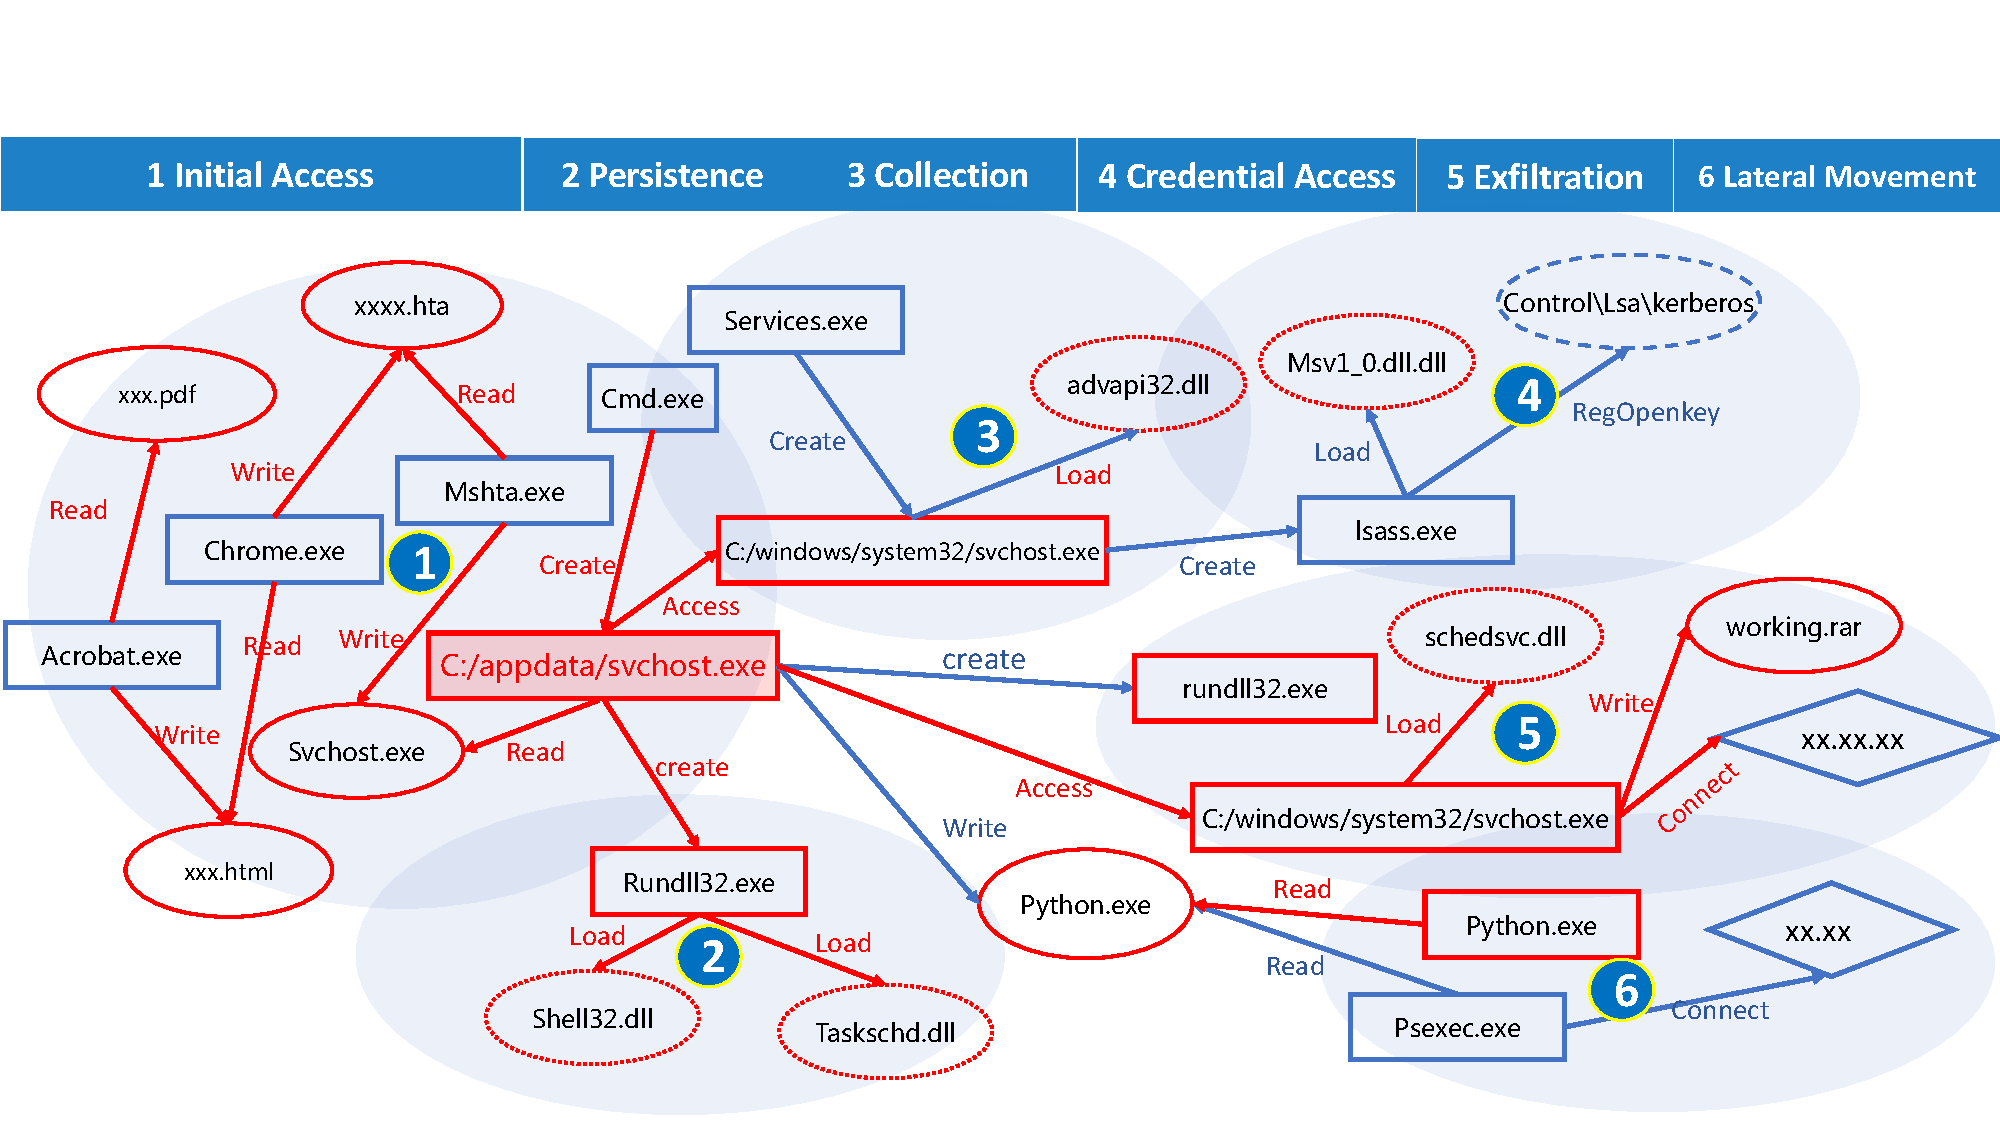
\includegraphics[width=0.9\textwidth]{figs/example.pdf}
    \caption{ 
    System entities are represented by nodes in the graph. 
    The attack-relevant elements are highlighted in red, while those representing regular events and nodes are displayed in blue.
    Processes, file-type entities (dlls, registry, files, etc.), and sockets are represented by rectangles, ovals, and diamonds. Solid line ovals represent files, dashed line ovals represent registries, and dotted line ovals represent DLLs. A series of operations is represented by an edge, such as read, create, and load. We have segmented the attack progression into six distinct steps using a light blue backdrop. }
    \label{fig-example}
    \end{figure*}

\paragraph{Attack Scenario}
Figure~\ref{fig-example} illustrates a simplified provenance graph derived from audit records of a trojan-induced APT attack. System entities are represented by nodes in the graph. 
Processes, file-type entities (dlls, registry, files, etc.), and sockets are represented by rectangles, ovals, and diamonds. Solid line ovals represent files, dashed line ovals represent registries, and dotted line ovals represent DLLs.
A series of operations is represented by an edge, such as read, create, and load.
There are 6 steps that are followed in the trojan-induced APT attack.
%In our analysis of APT attack reports \cite{eclecticiq2023,microsoft2023,paloaltonetworks2023}, we identify common attack steps and stealthy methods, such as Process Masquerade, Process Injection, Process Hollow, and DLL-Side Loading\cite{eclecticiq2023}. As a result of the use of four common obfuscation techniques, we were able to assemble ten scenarios for APT attacks using 23 malicious functions disguised as DLLs and program names.
%One of attack scenario as motivating example is used to illustrate current detection methods' limitations as well as our approach's intuition.


\begin{enumerate}[leftmargin=*]
    \item Initial Access: The attacker first sends the victim a malicious pdf file \textit{xxx.pdf} that contains a virus. Unfortunately, the application \textit{Acrobat.exe} that reads PDF files does not protect against the malicious code that is hidden inside the document. As a result, the malicious code downloads the malicious \textit{xxxx.hta} file, and the malicious program \textit{svchost.exe} is then downloaded and executed within the directory \textit{c:/appdata/svchost.exe}.
    \item Persistence: As an attempt to hide itself, this malicious \\ \textit{C:/appdata/svchost.exe} opens \textit{rundll32.exe}, which then uses a DLL Side-Loading technique to load a malicious DLL \textit{shell32.dll}, which contains functionality for establishing persistence in the compromised system.
    \item Collection: Malicious \textit{C:/appdata/svchost.exe} then injects malicious \textit{advapi32.dll} processes into a benign \\ \textit{C:/windows/system32/svchost.exe} and uses the malicious dll disguised as \textit{advapi32.dll} to gather information.
    \item Credential Access: Meanwhile, by exploiting a vulnerability, the attackers downgraded Kerberos to the more vulnerable NTLM protocol (\textit{Msv1\_0.dll}). In order to move lateral within the network, they stole credentials from the domain.
    \item Exfiltration: A malicious attacker hollows out a portion of the memory space of the benign process svchost, fills it with malicious programs, and packages up the information into a ZIP file known as \textit{working.rar}.
    \item Lateral movement: After obtaining the credentials from step 4, the attacker executed the renamed \textit{python.exe} file, thus gaining lateral access to the network.
\end{enumerate}




%\paragraph{Challenges to Existing Solutions}
%Our simulated APT attack shows the following limitations of provenance-based threat detection:
%\begin{itemize}[leftmargin=*]
%    \item \textit{Misuse-based Detection}:  A misuse-based detector\cite{milajerdi2019holmes,milajerdi2019poirot} detects cyber threats by matching audit records with security policies that describe attack semantics. The creation of these security policies is time-consuming and requires domain knowledge, even though such detection maintains a low false-positive rate. As shown in our example, a single TTP can correspond to a variety of different attacks, while "initial access" can be implemented in a variety of ways, our case utilizing \textit{Mshta.exe}. It is the responsibility of experts to cover all attack behaviors for a given TTP, but this is a time-consuming and labor-intensive process, and it cannot handle unknown or evolving threats. In addition, experts' subjective interpretations of attacks, varying proficiency levels, or even human error can affect the quality of policy formulation.
%    \item \textit{Anomaly-based Detection}: Anomaly-based detection techniques detect deviations, but they rarely provide a deeper understanding of the underlying attack mechanisms. Identifying the root cause of this attack scenario can be difficult due to the deluge of records generated by this attack scenario. As an example, Unicorn\cite{han2020unicorn} may trigger alerts across a graph, but it cannot pinpoint which particular entities or patterns are triggered. As a result of their ability to mimic benign activities, they are practically imperceptible, and in this attack scenario, many disguised behaviors can be seen. Process hollow is one of the disguised behaviors used in step 5. We get \textit{rundll32.exe} and the malicious \textit{svchost.exe} using the same vector based on Shadewatcher\cite{zengy2022shadewatcher}, so we cannot detect exceptions. Furthermore, the number of anomalous entries in benign logs is very low (less than 1\% of all entries are malicious). The limited representation of stealthy threats in logs makes it difficult to train a robust and reliable model.
%    \item \textit{Statistics-based Detection}: Even though statistics-based approaches \cite{liu2018towards,hassan2019nodoze,hassan2020we} identify potential threats within graphs, they often misinterpret benign but rare threats. For instance, in our motivating example, svchost has many functions, one of which hosts the schedule service. False alarms can occur due to infrequent incidents being flagged as attacks.
%\end{itemize}
%All of these methods have difficulties in identifying attacks in a timely and accurate manner. Further, they do not provide sufficient granularity to clarify and explain specific attack behaviors, which complicates the identification and response process in the event of an attack.



\paragraph{Our Solution}
\label{sec:intuition}
%As we mentioned previously, we analyze numerous APT attack
%reports\cite{eclecticiq2023,microsoft2023,paloaltonetworks2023} and discovered that attackers often employ disguise techniques to hide their malicious activities.
%The techniques include Process Masquerade, Process Injection, Process Hollow, and Direct Loading.
%It is generally true that as attackers progress from straightforward masquerading techniques, like mimicking legitimate processes, to more sophisticated ones, such as DLL\-side loading, the stealthiness of their disguises tends to increase.

In spite of the masquerading method, there are inherent behavioral invariant associated with genuine program behavior, regardless of the disguised method - execution paths, parent-child relationships, permissions, as a process must execute operations, some of which must be performed in sequence, etc.
To capture such constraints, we define behavioral invariants (see Section~\ref{sec:toolDefs} for more details) to limit the genuine program behaviors.
% Specifically, the behavioral invariants considered in this work are defined in Section~\ref{sec:toolDefs}:

% \fbox{
% \linyun{TODO: $p_1 \land p_2 \land ... $}
% }

However, there were significant deviations from these behavioral invariants. 
While \textit{svchost.exe} is typically spawned by \textit{services.exe}, the malicious variant here is spawned by \textit{cmd.exe}. Additionally, its execution path was not what one might expect for an authentic \textit{svchost.exe}.
For more stealth attacks, like process injection as shown in step 3, a maliciously injected \textit{advapi32.dll} disrupts the expected sequence of events and violates the associated constraints. Thus, it is essential that profiles and constraints are taken into account as detection signals for regular processes in order to improve detection capabilities.


% \fbox{
% \linyun{TODO:  $p_1 \land p_2 \land ... \land q_1$}
% }

% \linyun{$q_1$ for the runtime behaviors}


\section{Threat Model}\label{sec:threatModel}
We assume that APT attacks launch attacks with the following features:

\begin{itemize}[leftmargin=*]
    \item \textbf{Stealthy}. The attacker employs covert tactics, concealing their malicious activities amid a substantial volume of benign background data, resulting in the victim system exhibiting behavior akin to a benign mode.
    \item \textbf{Evolving}. Professional attacker groups continually innovate, extending their targets to a broader array of system processes and adeptly adjusting to the latest defensive mechanisms to maintain a competitive edge.
    %As professional attacker groups continue to innovate, they are targeting an ever-expanding range of system processes and adapting to the latest defensive measures in order to stay ahead of the game.
    \item \textbf{Frequent usage of zero-day exploits}. The attacker primarily relies on zero-day exploits, resulting in a lack of advanced knowledge w.r.t. the specific attack patterns.
\end{itemize}

\section{Methodology of \tool}

\begin{figure*}[ht]
    \centering
      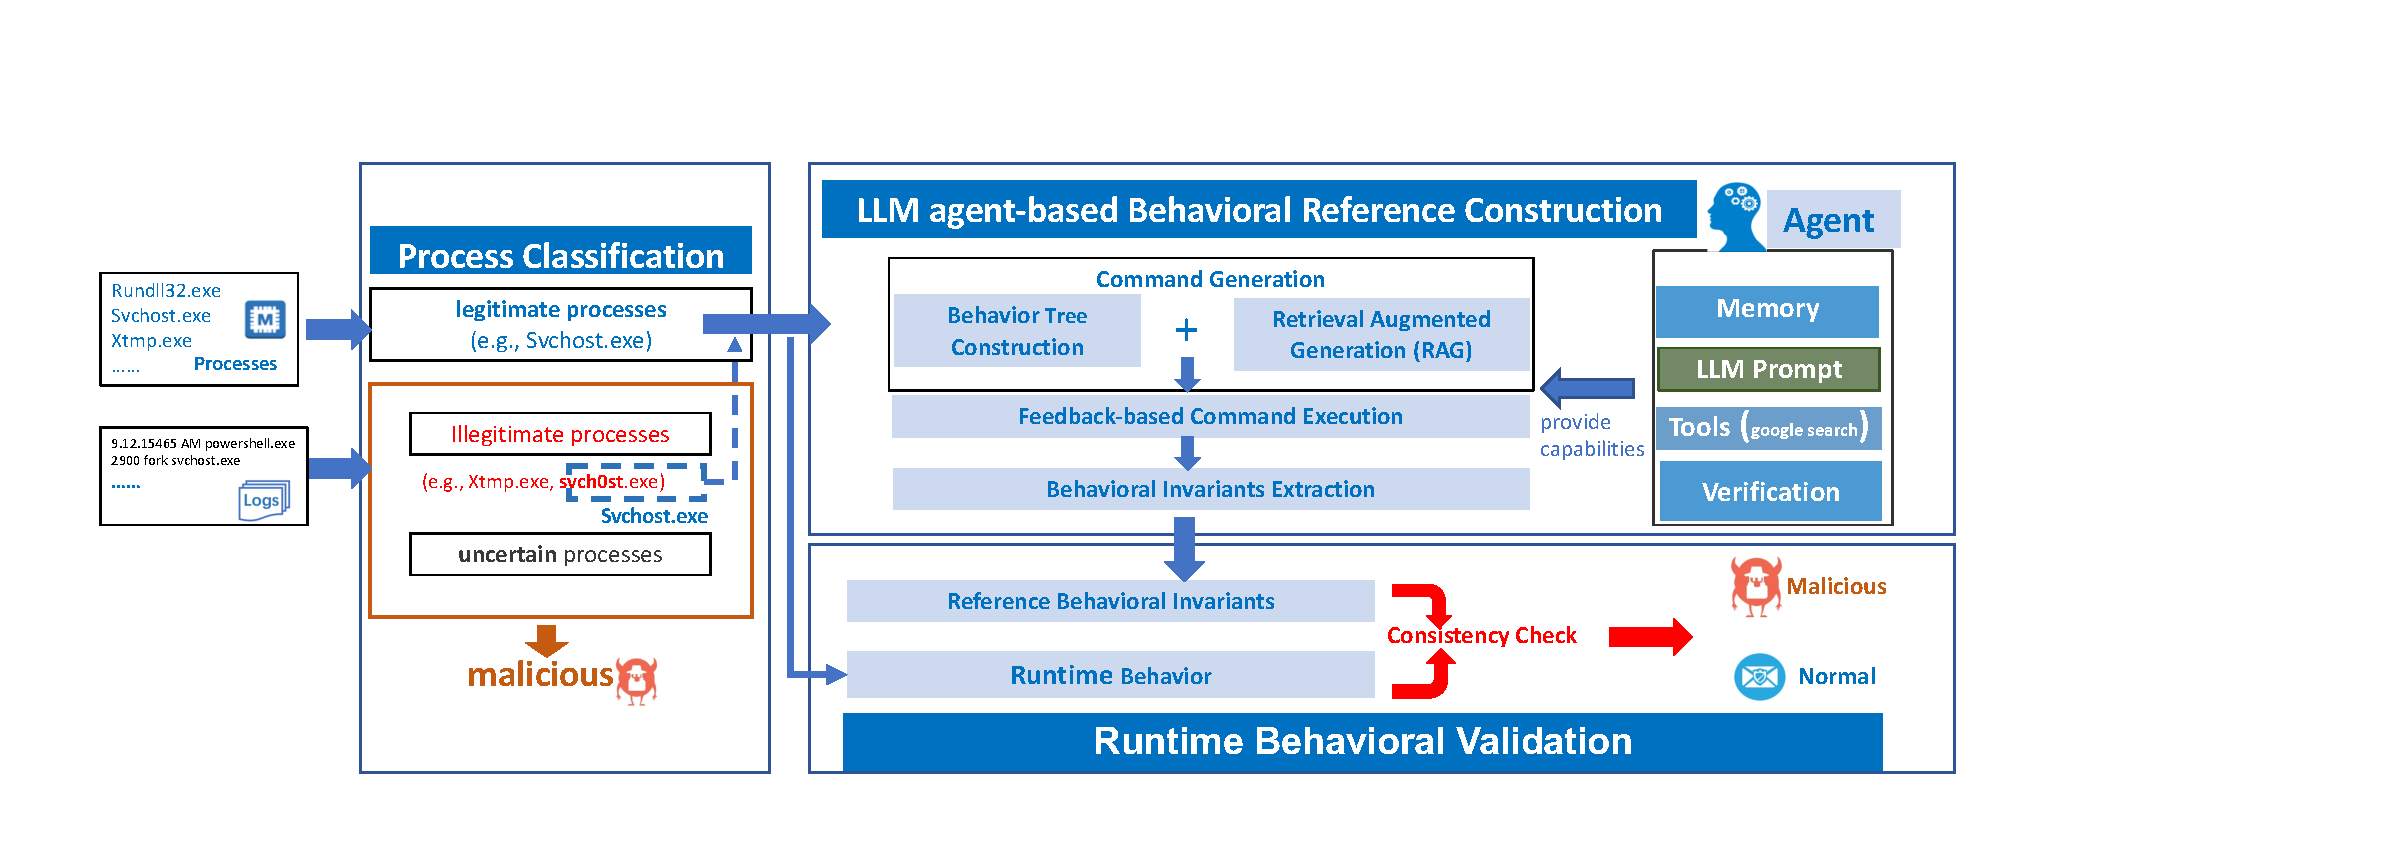
\includegraphics[width=0.85\textwidth]{figs/framework_new2.pdf}
      % \caption{An overview of \tool.}
    \caption{An overview of \tool. }
    %Given a bundle of logs collected from system processes, \tool first filters legitimate processes as detection targets while regarding the others as potential malicious attacks. Then, \tool constructs a behavioral invariant for each legitimate process via the Behavioral Reference Construction Module, which is in the form of disjunction and/or conjunction of reference propositions. Finally, the Runtime Behavioral Validation module will transform both the behavioral invariants generated before and the original runtime systems logs into sets of logical propositions for the target processes, respectively. By checking the consistency of two sets of propositions (e.g., checking the satisfiability of the conjunction of all propositions from the two sets), \tool will return the detection result.}
    \label{fig-framework}
\end{figure*}


\subsection{Technical Challenges}\label{sec:challenges}
A straightforward idea is to utilize the knowledge extraction capabilities in LLMs to facilitate the construction of more comprehensive behavioral invariants for victim system processes first, which can then be employed for conducting further thorough attack detection analysis. Recall that,
when dealing with the evolution of attacks or their stealthy tactics, supplemental knowledge can be very crucial. Moreover, in contrast to learning-based detection methods, this approach obviates the requirement for pre-defined attack patterns, which also enhances its adaptability and versatility in addressing evolving threat landscapes.
However, the direct employment of LLMs in our setting gives rise to the following three notable technical challenges:

\noindent
{\bf CH-\circled{1} Context Dependency.} %  :
LLMs' ability to extract process behavior knowledge heavily relies on the context provided in the input. Without sufficient context or in cases of ambiguous information, LLMs struggle to generate rich and accurate behavior descriptions. This limitation is significant in complex domains where behaviors are intricately linked to specific circumstances or prerequisites.

\noindent
{\bf CH-\circled{2} Provision of Outdated Information.} % \circled{2}
The dynamic nature of knowledge means that documentation and processes are regularly updated. However, LLMs might not be immediately updated to reflect these changes, leading to the provision of information that is outdated and potentially misleading.

\noindent
{\bf CH-\circled{3} Hallucination Issues.} % \circled{3}
Hallucination in LLMs refers to the generation of information that is not based on the input data or grounded in reality. This includes providing false information in the absence of clear answers and creating responses based on non-authoritative or unreliable sources.


\subsection{Overview of \tool}
In this work, we propose an effective LLMs-based APT attack detection framework, named \tool, addressing all the above challenges. The overview of \tool can be found in Figure~\ref{fig-framework}.

\tool comprises three main modules: Process Classification, Behavioral Invariants Construction, and Runtime Behavioral Validation. Given a bundle of logs collected from system processes, \tool first filters legitimate processes as detection targets while regarding the others as potential malicious attacks. Then, the Behavioral Reference Construction Module constructs a behavioral invariant for each authorized process, specifically utilizing a structure composed of facts and temporal behavioral invariant. Finally, the Runtime Behavioral Validation module transforms both the previously generated behavioral invariants and the original runtime system logs into a logical framework for the target processes, respectively. By evaluating the consistency between the reference and runtime invariants, the tool determines the detection outcome, where consistency indicates normal behavior and inconsistency signifies malicious activity.

Specifically, to address the technical challenges outlined in Section~\ref{sec:challenges}, We employ the LLM agent architecture to fully harness the capabilities of both LLMs and traditional software for constructing the Behavioral Reference as shown in Figure~\ref{fig-framework}.


\noindent
{\bf Process Behavior Tree Construction.} To provide an enriched contextual environment for LLMs, we first capture a comprehensive range of behaviors for each process, i.e., creating a behavior tree for each process. Then, the Large Language Models (LLM) continuously expands its knowledge of this behavior tree through a ``self-ask'' manner. Finally, the LLM benefits greatly from this behavior tree as it provides an enriched contextual environment, which can greatly tackle {\bf CH-\circled{1}}.

\noindent
{\bf Retrieval Augmented Generation.} 
To address challenges related to outdated information and the reliability of knowledge, we employ a Retrieval Augmented Generation (RAG) module. This module initially conducts a Google search to obtain the top $N$ documents relevant to the topic at hand. It then utilizes these documents to construct additional commands. These newly generated commands are integrated with those produced in the initial step, facilitating the acquisition of more current and authoritative knowledge. This approach primarily aims to overcome the {\bf CH-\circled{2}} and {\bf CH-\circled{3}} by ensuring the information provided is both up-to-date and credible.


\noindent
{\bf Feedback-based Command Execution.} 
Our third step involves executing the commands generated in the first two steps within the system. To address {\bf CH-\circled{3}}, we implement a feedback execution update mechanism. Initially, if the commands encounter execution challenges such as missing parameters, files, or parameter dependencies, these issues are directly fed back to the LLM, which then updates the current commands accordingly. Following the execution, actual logs are obtained, which are used for subsequent steps. This method ensures that execution hurdles are promptly identified and rectified, leading to a more efficient and error-free operation.

\noindent
{\bf Behavioral Invariants Extraction.} In the final step, we first employ common term and prefix-span sequence mining algorithm to unearth deeper relationships within the logs. Subsequently, LLMs are utilized to interpret these invariants, providing insights into the underlying patterns and associations. This integrated approach not only maximizes the strengths of both methodologies but also facilitates a comprehensive analysis of the logs, leading to a richer understanding of the data.







\section{Design of \tool}

\subsection{Definitions}\label{sec:toolDefs}
\noindent
{\bf System Entity.} In this work, we distinguish five principal entity categories: \textit{Processes}, \textit{Files}, \textit{Registry}, \textit{Dynamic Link Libraries (DLLs)}, and \textit{Network Connections}, the latter typically denoted by sockets. System entities possess unique attributes: the attributes associated with \textit{process} entities might include their Process ID (pid) or their executable paths. 

\noindent
{\bf System Event.} In this work, a system event $e$ is given by a tuple $\langle src, dst, rel, time\rangle$, where $src$ designates the source entity, constrained to only process entities, $dst$ indicates the target or destination entity, $rel$ denotes their interaction nature (e.g., writing into a file), and $time$ specifies the timestamp of the event occurrence.
We also illustrated the temporal relationship between events as $\langle e_1 \to e_2 \to e_3 \rangle$, indicating that the events occur in a logical sequence. 

% \noindent
% {\bf Proposition Definition.}
% A proposition is represented as a triplet $\langle src, operation, dst\rangle$, where:
% \begin{itemize}
%     \item $src$ and $dst$ represent entities.
%     \item Entities can be: Process, Dll, Registry, File, IP:port.
%     \item An operation is performed from the $src$ to the $dst$.
% \end{itemize}

\noindent
{\bf Behavioral Invariant.} In this work, the behavioral invariant is defined as follows:
\begin{align*}
 & \mathcal{I}  ::= \ \phi \mid \phi \wedge \mathcal{I} \\
 & \phi  \ \ \in \ \{ P_{ep}(x,y), \ P_{pp}(x,Y), \ P_{cp}(x,Y), \ P_{a}(x,y), \ P_{o}(x_1,x_2,\ldots)\} \\
\end{align*}
where $P_{ep}(x,y)$ (resp. $P_{pp}(x,y)$) indicates that the execution path (parent process) of process $x$ is $y$, $P_{cp}(x, Y)$ indicates that the child processes of $x$ must come from processes set $Y$, $P_{a}(x,y)$ denotes that the process $x$ must execute the action $y$ in the future, and the $P_{o}(x_1,x_2,\ldots)$ requires that the processes must be executed in the sequential order of $x_1,x_2,\ldots$.

For example, a behavior invariant $\mathcal{I}_e$ of \texttt{svchost.exe} can be represented by the conjunction of the following set: 

\begin{center}
$ \left\{
\begin{array}{c}
P_{ep}(\texttt{svchost.exe}, \text{``C:/windows/system32/''}),\\
 P_{pp}(\texttt{svchost.exe}, \texttt{services.exe}),\\
 P_{a}(\texttt{svchost.exe}, \text{Load(\texttt{advapi32.dll})})
\end{array} \right\}$
\end{center}

which states that the execution path of \texttt{svchost.exe} should be \text{"C:/windows/system32/"}, with parent process 
as \texttt{services.exe}, and it will load \texttt{advapi32.dll} finally.


\subsection{Process Classification}
We created a prompt to query LLMs that classified these processes into legitimate, illegitimate, and uncertain names (due to the LLMs database's incompleteness).
Due to name confusion, many illegitimate process names can be changed to legitimate process names for further evaluation.
For both the legitimate and confusion processes, we construct profiles according to the methods described in the following sections. An investigator should investigate further illegitimate or unclear categories since they may contain malware.


\subsection{Behavioral Reference Construction}
In this section, we describe the methodology for constructing Behavioral References for processes, which can be categorized into three phases. 
This method combines the strengths of Language Model (LLM) agents, particularly utilizing Retrieval Augmented Generation (RAG) and Direct Query LLMs, to create accurate and diverse command sets, sandbox testing environments for empirical validation, and algorithmic extraction of behavioral invariants based on common and frequent item mining. The framework aims to mitigate the phenomenon of "hallucinations" in LLM outputs through a multifaceted validation strategy.


\subsubsection{Retrieval Augmented Generation (RAG)}
To generate accurate command sets, we first implement the Retrieval Augmented Generation (RAG) method, and second, to generate a more diverse, we utilize Direct Querying of LLMs for the generation of process behavior trees. Together, these two steps collaborate to produce accurate and diversified commands.

\noindent
{\bf Utilizing Search Engines}: Initially, the RAG system employs a search engine, such as Google, to perform a broad and comprehensive search based on the user's query. This step is about casting a wide net to ensure no relevant document is overlooked.

\noindent
{\bf Retrieving Top Documents}: From the search results, the system selects the top $N$ documents. The selection criteria hinge on relevance to the query, recency, and the credibility of the sources. These documents are pre-indexed in a database that the RAG system can query.

\noindent
{\bf Indexing for Quick Access}: Each document is broken down into manageable chunks or vectors, with key concepts and information encoded into embeddings. These embeddings act as a map to the knowledge landscape within each document, allowing for rapid and efficient retrieval of information.

\noindent
{\bf Indexing and Retrieval}: The RAG system begins by searching through a pre-indexed database of documents to find chunks of text relevant to the user's query based on the prompt as shown in Appendix~\ref{prompt-rag-commands}. This is analogous to sourcing current and contextual data that can inform the behavior of the process.

\noindent
{\bf Command Generation through Contextual Relevance}: The system then retrieves documents that appear to have the highest relevance to the process in question. For instance, in a process related to data privacy, RAG might retrieve the latest legal regulations, industry best practices, and recent case studies.


\subsubsection{Process Behavior Tree Construction}
The construction of \textit{Process Behavior Trees} is one of the most important steps in the process.
First, we define the \textit{Process Behavior Tree}.
\begin{figure}[h]
    \centering
      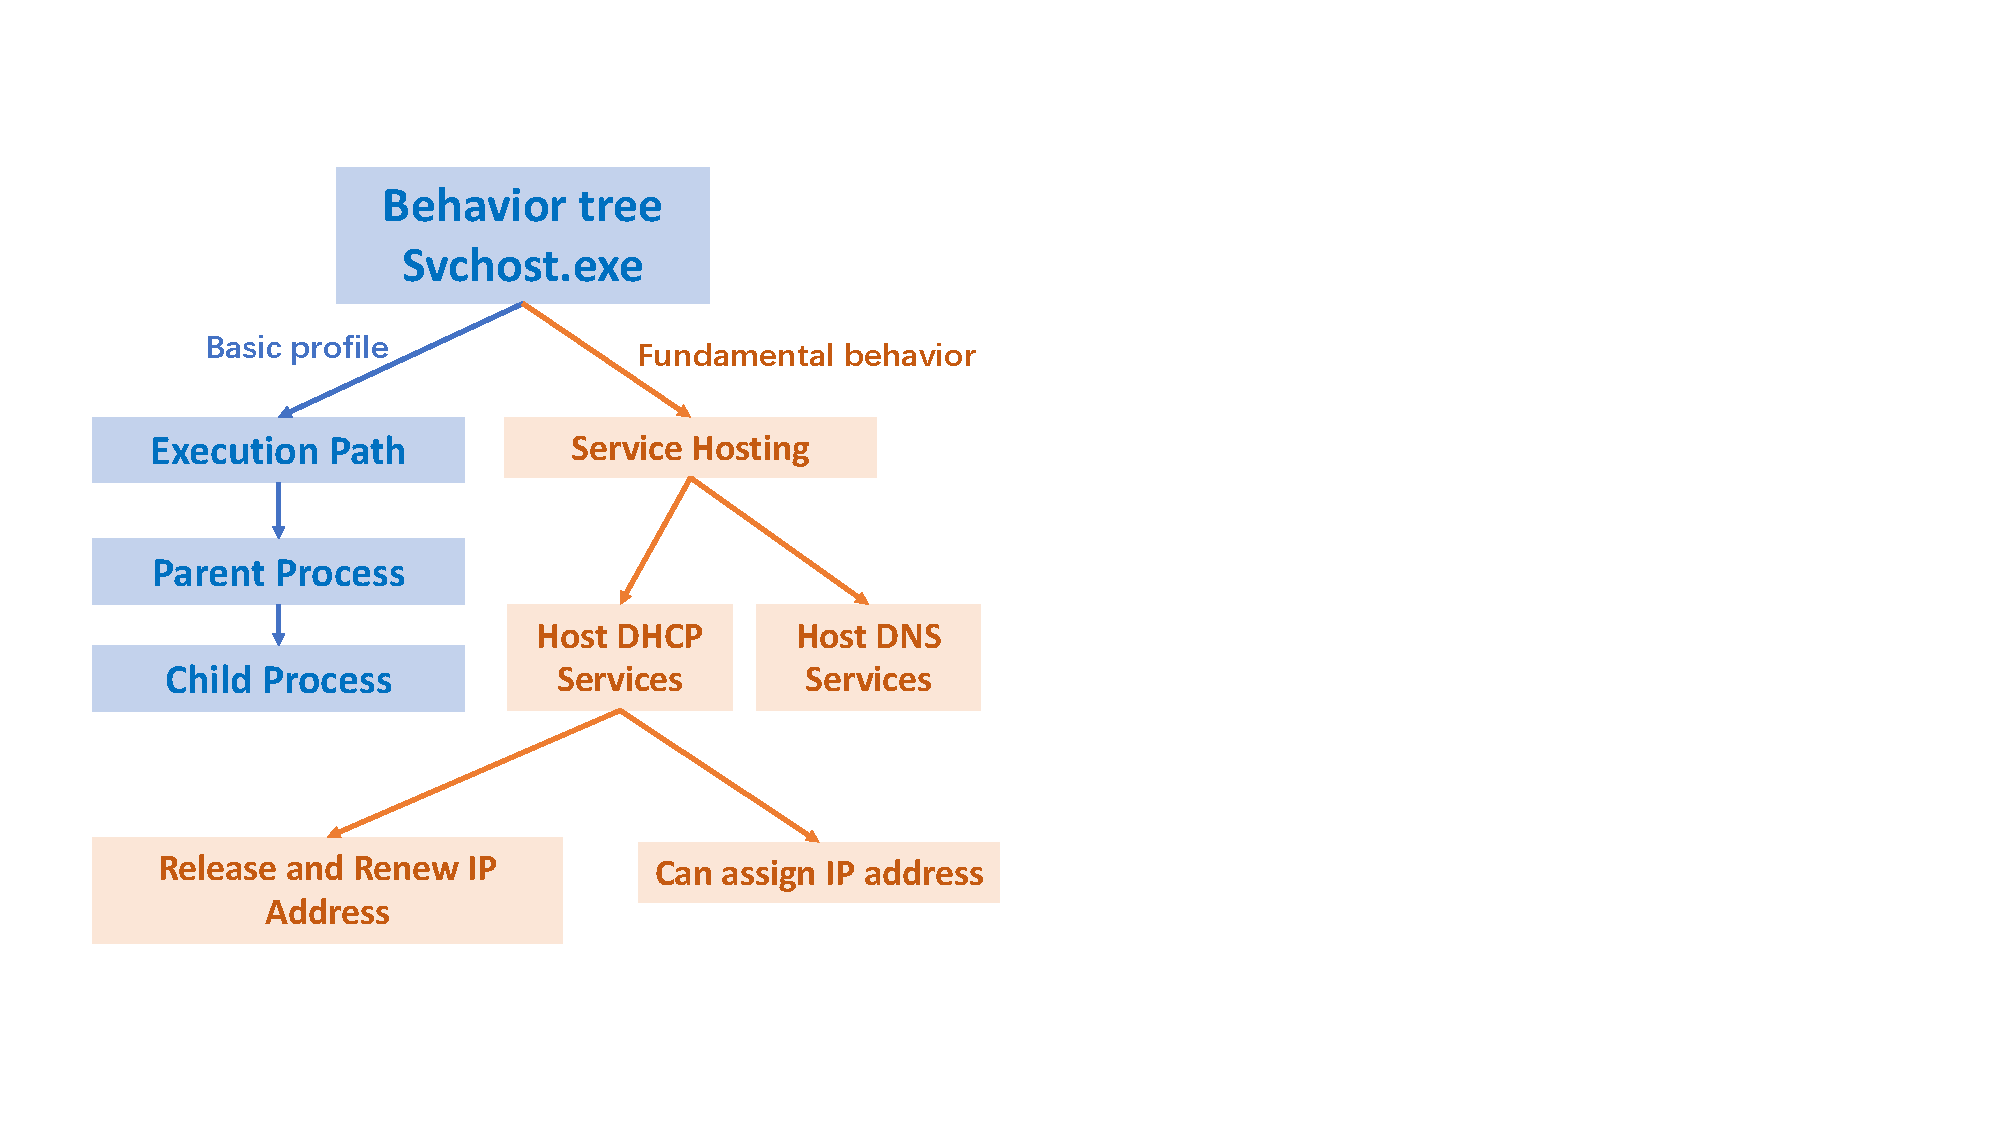
\includegraphics[width=0.35\textwidth]{figs/tree1.pdf}
    \caption{Process Behavior Tree Representation.}
    \label{fig:BT}
\end{figure}

To generate as many behaviors as possible, we've crafted two prompts: the \textit{Initialization Behavior Tree Prompt}(A detailed prompt can be found in the Appendix~\ref{prompt-init-tree}) and the \textit{Expansion Behavior Tree Prompt}. Initially, we employ the \textit{Initialization Behavior Tree Prompt} to create a foundational behavior tree. Subsequently, this tree is expanded through iterative rounds using the \textit{Expansion Behavior Tree Prompt}.

The resulting behavior tree is illustrated in Figure~\ref{fig:BT}. Taking the behavior tree of \textit{svchost.exe} as an example, we begin with the basic profile. This includes details such as the execution path of the process, its parent process (the parent process of \textit{svchost.exe} can only be \textit{services.exe}), and its child processes. Following this, we have the fundamental behaviors, such as service hosting, DLL loading, and service isolation exhibited by \textit{svchost.exe}. Focusing on the most significant behavior, which is service hosting, the behavior tree can be extended to detail the specific services being hosted. 

\subsubsection{Feedback-based Command Execution}
Following command generation, the next step involves the creation of an automated sandbox testing environment. Within this environment, the generated commands are executed, and logs for each command's behavior are collected. These logs serve as the foundation for the subsequent extraction of behavioral invariants, facilitating a deeper understanding of the process's dynamics and ensuring the commands' validity.

The stage of command execution is a critical juncture in the process of Behavioral Reference Construction, where the practical viability of generated commands is put to the test. This phase involves a sophisticated feedback loop within an automated sandbox testing environment to refine and perfect the command set for assured success upon execution.

\noindent
{\bf Execution in Automated Sandbox}:
An automated sandbox environment is set up to provide an isolated testing ground for the execution of commands, simulating actual operational conditions while protecting the main system from potential negative impacts of untested commands. During this phase, commands generated earlier are input into the sandbox, where each command's execution is meticulously monitored, with the system recording its behavior, results, and any errors that occur.

\noindent
{\bf Error Feedback Mechanism}:
In the quest for precision, the execution phase includes an error feedback mechanism to address failures in command execution from the previous stage. Common errors identified involve incompatible parameter combinations, such as using -h for file or printer sharing with -k for registry keys, which targets incompatible objects. There are also instances of misformatted commands, like pairing -f, which displays full process token information, with -c for Windows services, leading to a context mismatch. Additionally, issues with erroneous or missing parameter values are frequent, such as a command where -f is used without an accompanying account list after -p for specifying a process name or PID. To rectify these issues, an error correction loop is formed, leveraging both the LLM and sandbox outputs to iteratively refine commands. This loop represents a dynamic interplay between the LLM's generative abilities and the empirical data from the sandbox, substantially improving the success rate of command executions.

\noindent
{\bf Knowledge Augmentation Feedback}:
To enhance command generation further, the system integrates feedback on the relationships between parameters, including conflicts and dependencies. Conflicts arise when certain parameters, like -h and -k or -p and -c, cannot coexist due to their differing object applications. Conversely, dependencies are noted where parameters should be used together, such as -l with -i for displaying security descriptors excluding inherited ACEs, or -f with -p for full process token information. Through this systematic refinement, the system strengthens its grasp on parameter conflicts and dependencies, significantly boosting the accuracy of command generation by ensuring that only compatible and contextually relevant parameters are paired.



\subsubsection{Behavioral Invariants Extraction}

The final phase of the framework focuses on extracting Behavioral Invariants using algorithms for mining common and frequent items. This step leverages both traditional algorithms and the interpretive capabilities of LLMs to identify invariant behaviors within processes, enhancing the robustness of the Behavioral Reference Construction.

\begin{figure*}[h]
  \begin{subfigure}{.45\textwidth}
      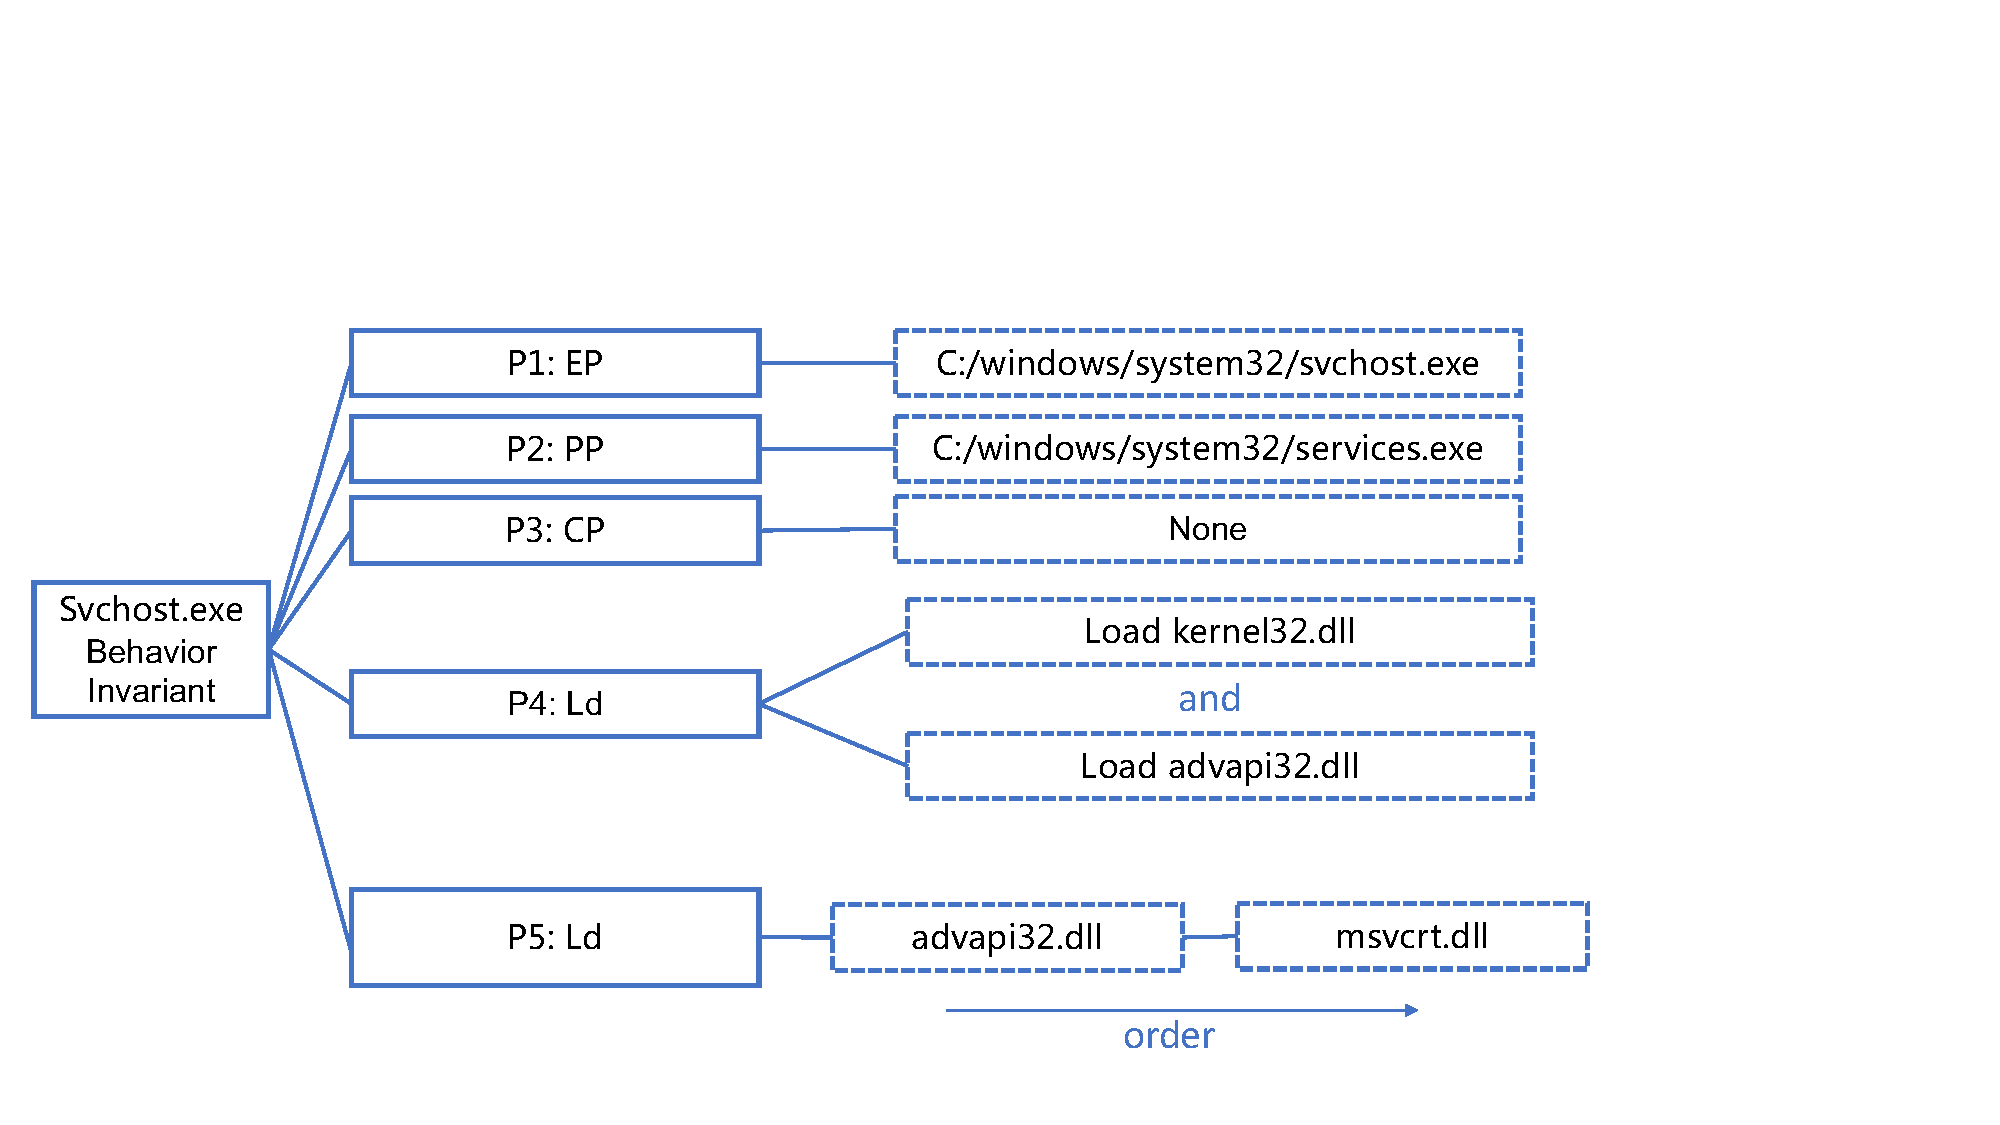
\includegraphics[width=\textwidth]{figs/cons-svchost.pdf}
      \caption{Behavioral Invariants of Svchost}
      \label{fig:cons-svchost}
  \end{subfigure}
  \hfill
  \begin{subfigure}{.5\textwidth}
      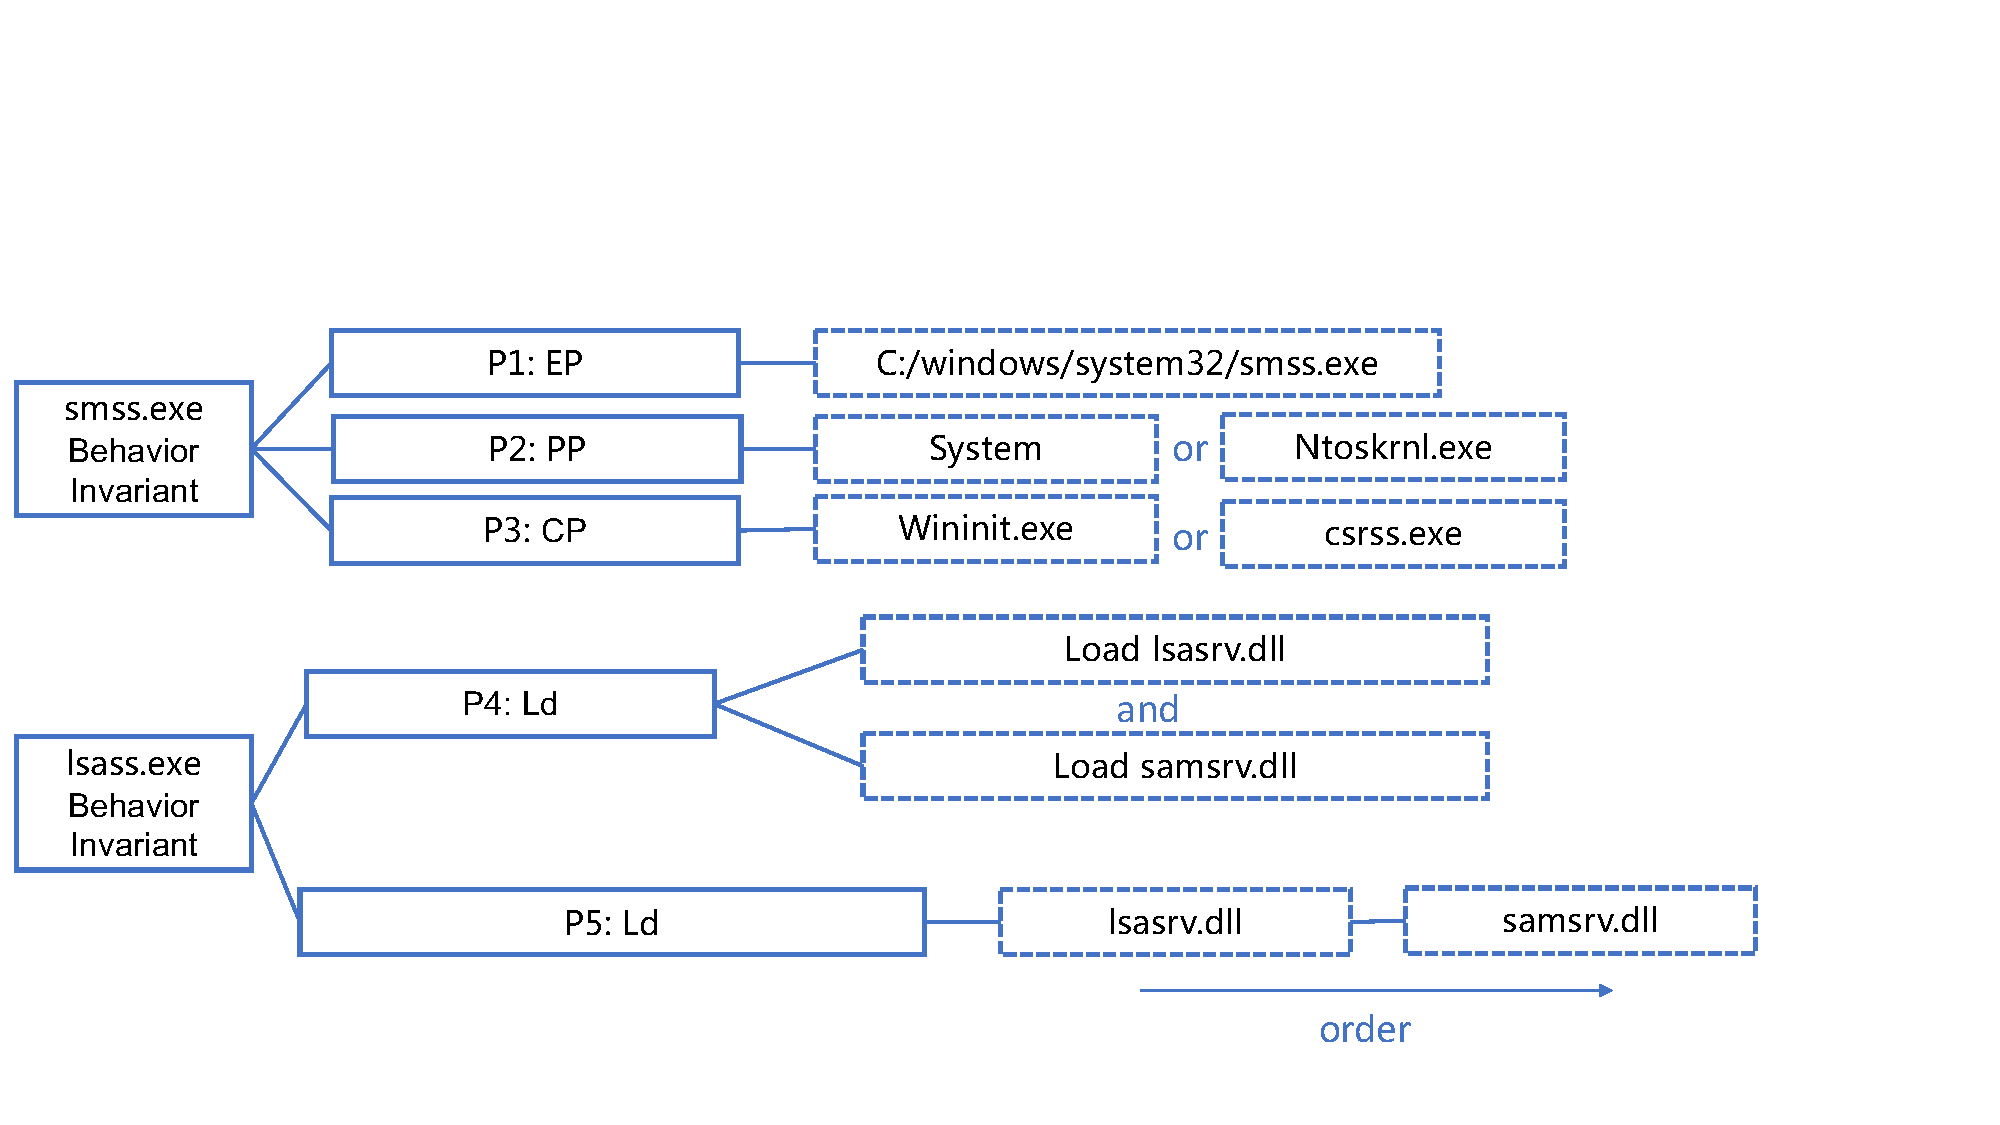
\includegraphics[width=\textwidth]{figs/cons-smss-lsass.pdf}
      \caption{Behavioral Invariants of Smss and Lsass}
      \label{fig:cons-smss-lsass}
  \end{subfigure}
  \hfill
  \caption{Behavioral Invariants: 'EP' stands for Execution Path, 'PP' represents Parent Process, 'CP' is for Child Process, and 'LD' refers to Load.}
  \label{fig:cons-def}
 \end{figure*}

The extraction of process behavioral invariants is a pivotal step in our methodology. We begin by categorizing behavioral invariants into five types as shown in Figure~\ref{fig:cons-def}.
The Figure~\ref{fig:cons-def} illustrates the behavioral invariants of three processes: \textit{svchost.exe}, \textit{lsass.exe}, and \textit{smss.exe}. In Figure~\ref{fig:cons-svchost}, the behavioral invariants of \textit{svchost.exe} are shown. There are five types of behavioral invariants: execution path, parent process, child process, intrinsic behavioral invariants (\textit{svchost.exe} will always load \textit{kernel32.dll} and \textit{advapi32.dll}.), and temporal behavioral invariants (\textit{advapi32.dll}, \textit{msvct.dll}, and \textit{kernelbase.dll} must be loaded in the specified sequence).
For certain processes, like \textit{smss.exe}, parent and child processes are optional. The parent process of \textit{smss.exe} can be \textit{system} or \textit{Ntoskml.exe}.

By comparing them with the logs gathered in the previous steps, we can validate and extract the first three behavioral invariants directly.
However, for intrinsic and temporal behavioral invariants, the challenge arises due to real-world logs' vastness. It is impractical to query the LLMs for each log due to memory constraints and its propensity to forget extended conversations. To overcome this, we designed a hybrid method that combines traditional programming techniques with queries to the LLMs to extract these two behavioral invariants.

We want to identify behaviors that are certain to occur in a specific process and in a certain order. 
We begin by mining the logs for common items among different log sequences.   
To speed up common sequence mining, we removed content from sequences that do not include common items when getting common items.
our next step is to use the PrefixSpan algorithm to find common sequences in these logs. 
To obtain the common sequences, rather than frequent sequences, we set the threshold \( \theta =1\) of the PrefixSpan algorithm, indicating that the sequence is certain to occur in the specified order.
(Algorithms are detailed in the Appendix~\ref{alg:fre-common}.
Having established the common items and sequences, we then direct our queries towards the LLMs, focusing specifically on these elements to extract intrinsic and temporal behavioral invariants. 
The detailed set of prompts used in this process is shown in Appendix~\ref{prompt-cons-explain}.

Furthermore, we request the LLMs to explain its findings, providing insights into these behavioral invariants.
Based on the prompt as shown in Appendix~\ref{prompt-cons-explain}, we ask LLMs to explain why this behavioral invariant exists, such as why \textit{lsass.exe} must load \textit{lsasrv.dll}, and why \textit{lsass.exe} must load \textit{samsrv.dll} after loading \textit{lsasrv.dll}. 
The LLMs would respond: \textit{lsass.exe} loads \textit{lsasrv.dll} primarily to utilize its code to complete tasks such as authentication and the generation of security tokens. 
\textit{lsass.exe} loads \textit{samsrv.dll} to manage and access the security account database, supporting user authentication and the implementation of local security policies


\subsubsection{Combating LLM Hallucinations}
The framework adopts a three-pronged approach to address and mitigate the issue of hallucinations in LLM outputs:

\begin{itemize}
    \item \textbf{Verification through RAG}: By validating commands against real-world documents, RAG ensures the accuracy and relevance of the generated commands.
    \item \textbf{Empirical Validation in Sandbox}: Executing commands within a sandbox environment serves as a practical verification step, ensuring the commands operate as intended.
    \item \textbf{Multi-Agent Debating}:Employing a multi-agent debate strategy further guarantees the correctness of LLM outputs, providing a comprehensive check against potential errors.
\end{itemize}

The LLMs engage in iterative debates in multiple instances. Their goal is to find a consensus on an answer that is both accurate and reliable by verifying each other's responses and reasoning. They cannot reach a consensus on actions that are not entirely correct by having multiple LLMs debate each other. For definitive behaviors, they can eventually come to an agreement. A more detailed description of our approach can be found in the Appendix~\ref{prompt-cross-validation}.


\subsection{Runtime Behavioral Validation}
During this phase, we focus on a systematic comparison between the behavioral invariants, formulated by the Behavioral Reference Construction module, and the actual behaviors manifested during the system's runtime.

The behavioral invariants are identified through a combination of multiple criteria, extracted to create a reference framework. We analyze the behaviors captured in the system logs using a methodology akin to that described in the "Behavioral Invariants Extraction" section. This process enables us to establish a comprehensive framework of behavioral norms based on the original system logs, which helps us identify key conditions that are indicative of expected runtime behavior.

The critical step involves conducting an in-depth analysis of consistency between these expected behavioral conditions and the actual observed system behavior. This step is crucial as any discrepancy from the established invariants is considered a potential sign of malicious activity. By evaluating the consistency between the reference behavioral invariants and runtime behaviors, the tool determines the detection outcome. Here, consistency correlates with normal behavior, while inconsistency points to potential malicious activities.
\section{Experiment Evaluation}

In order to validate the effectiveness of our approach, we conducted a series of simulations. Four common trojan stealth techniques were replicated. We also simulated 23 malicious function attacks frequently used by Trojan programs, targeting 70 critical system processes. Additionally, ten Trojan-based APT attack scenarios were also executed as part of our comprehensive evaluation.

\begin{itemize}
    \item \textbf{Q1.} How well does our method work, and does it achieve a low false-positive rate and low false-negative rate? (§~\ref{sec-effective})
    \item \textbf{Q2.} What is the time it takes for our method to construct a profile for each process? What is the most time-consuming step in the three-step process profile creation? (§~\ref{sec-eff})
    \item \textbf{Q3.} How does the behavior diverge based on LLM, and how does the validation step optimize the outcome? (§~\ref{sec-ab-study})
    \item \textbf{Q4.} How can we validate the accuracy of these explanations using our method? (§~\ref{sec-explanation-val})
    \item \textbf{Q5.} Is it common for real-world APT attacks to disguise their processes in various ways? (§~\ref{sec-real-world})
\end{itemize}


\subsection{Implementation}
All experiments are performed on a server with AMD EPYC 7543P 32-Core Processor, 256 GB physical memory. The OS is Microsoft Windows 10 (64-bit).
We implemented our system by calling OpenAI's GPT-4 API with a temperature setting of 0.5.
We developed \tool in 3.53K lines of C++ code and 10K lines of Python code.

\paragraph{System Auditing Collection.}
Although \tool can handle input from Linux and Windows systems, our evaluation focuses primarily on Windows events. Because most of our benign deployment environment consists of Windows-based hosts, and sophisticated malware is mostly designed for Windows platforms.
We use \textit{Sysmon}, Windows's log collection tool, to collect provenance data from these systems.

\subsubsection{Attack Datasets}

To address the challenges, we approached the problem from three distinct angles: expanding coverage of malicious functionalities and the ATT\&CK framework, employing trojan stealth techniques, and simulating Trojan-based APT attacks.

We executed Trojan-based APT attack simulations in three steps:
\begin{itemize}
    \item \textbf{Enhancing Malicious Functionalities}: In order to simulate a wider range of malicious function attacks frequently used by Trojan programs, we handcrafted 23 malicious functions in C++ and \textit{Caldera}\cite{caldera}, including BypassUAC, File Scan, File Monitor, Compression, Keyboard Monitor, and Privilege Escalation. In addition, we implemented 9 different TTP attacks using well-known hacker utilities. 
    \item \textbf{Employing Stealth Techniques}: We incorporated Four common trojan stealth techniques: Process Masquerade, Process Hollow, Process Injection, and DLL Side-Loading. By combining these stealthy techniques with the 23 malicious functionalities, we created a variety of attack variants. 
    \item \textbf{Simulating Real-world APTs}: In order to enhance the authenticity of our simulations, we developed ten Trojan-based APT attack scenarios based on an analysis of real-world trojan-based APT activities. We crafted ten simulated APT attack narratives using the four stealth techniques from the second step and the 23 malicious functionalities from the first step.
\end{itemize}

% \noindent
% {\bf DARPA Datasets.} We used data from DARPA’s Transparent Computing (TC) and Operationally Transparent Cyber (OpTC) programs, featuring simulated APT attacks on enterprise networks and benign activities. The TC dataset includes attacks on critical services and benign operations, with data captured by various systems. The OpTC dataset covers benign and mixed APT activities over ten days on Windows hosts. From these, we specifically extracted scenarios involving the use of obfuscation techniques.

\noindent
{\bf Real-world datasets.} Using real-world Trojan-based APT datasets, we aimed to validate the frequency of masquerade techniques such as name masquerading in authentic APT attacks; to this end, we collected publicly available APT attack simulation datasets alongside malware samples like GALLIUM\cite{cybereason2023}, DCSrv\cite{checkpoint2021},  which are known to employ techniques like name masquerading and process injection;  APT29 poses as \textit{python.exe}, \textit{rar.exe}, and \textit{accesschk.exe}; furthermore, they utilize DLL Side-Loading, specifically by loading a malicious \textit{mso.dll} file, with comprehensive details showcased in Table~\ref{tab:real_world}.


\noindent
{\bf Label.}
By using our knowledge of attack workflow, we manually label the ground truth of interactions through their relation to attacks, as we are aware of how attacks are executed.


\subsubsection{Normal Datasets}
To validate the false positive rate of our methodology, a publicly available benign dataset \cite{evtx-baseline2022} is used in this analysis. This dataset encompasses logs generated from routine user activities across various Windows operating systems, including Windows 7, Windows 10, and Windows 11. The logs from this dataset cover 13/47/52 processes for different systems that we used to construct process profiles.

\subsubsection{Process Classification}
We carefully selected 70 important processes based on various criteria: 1) Essential system processes; 2) Processes closely related to security mechanisms; and 3) Processes often used by system administrators. 

The two most common camouflaged processes are \textit{svchost.exe} and \textit{rundll32.exe}:
\begin{itemize}
    \item \textit{Svchost.exe} processes. \textit{svchost.exe} is a Windows system utility that runs multiple services from dynamic link libraries (\textit{dll} files). Trojan malware can easily masquerade as \textit{svchost.exe} \cite{svchost2023}.
    \item \textit{Rundll32.exe} processes. \textit{rundll32.exe} loads specific functions from \textit{dll} files. Unlike \textit{svchost.exe}, it's more vulnerable, as attackers can create their own \textit{dll} for it. Due to its exploitability, \textit{rundll32.exe} is a prime target for trojan impersonation. 
\end{itemize}


\subsection{Effectiveness}
\label{sec-effective}

\begin{figure*}
  \centering
  \begin{minipage}[b]{0.65\textwidth} 
  \begin{subfigure}{.5\textwidth}
      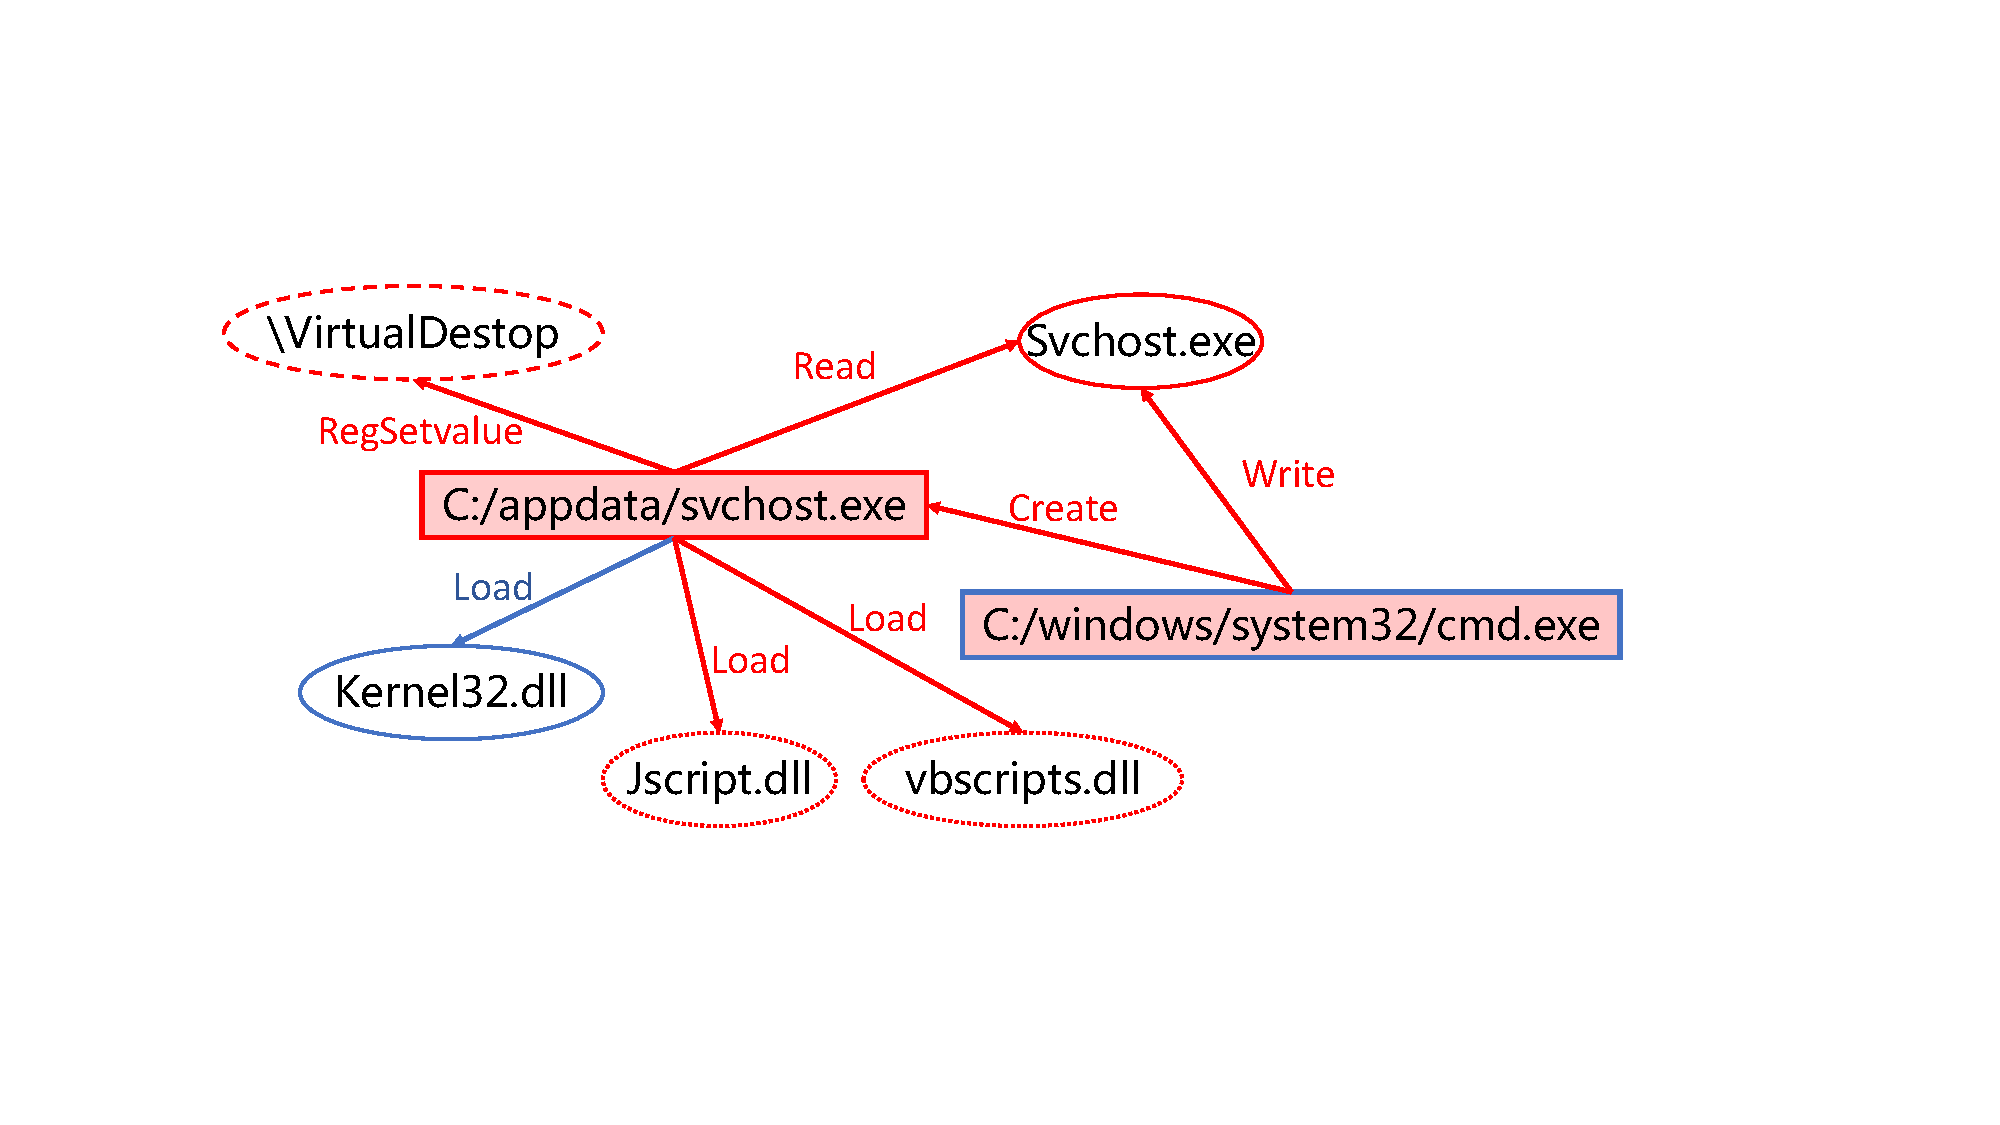
\includegraphics[width=\textwidth]{figs/Process Masquerade.pdf}
      \caption{Process Masquerade}
      \label{fig:process_mas}

  \end{subfigure}
  \hfill
  \begin{subfigure}{.5\textwidth}
      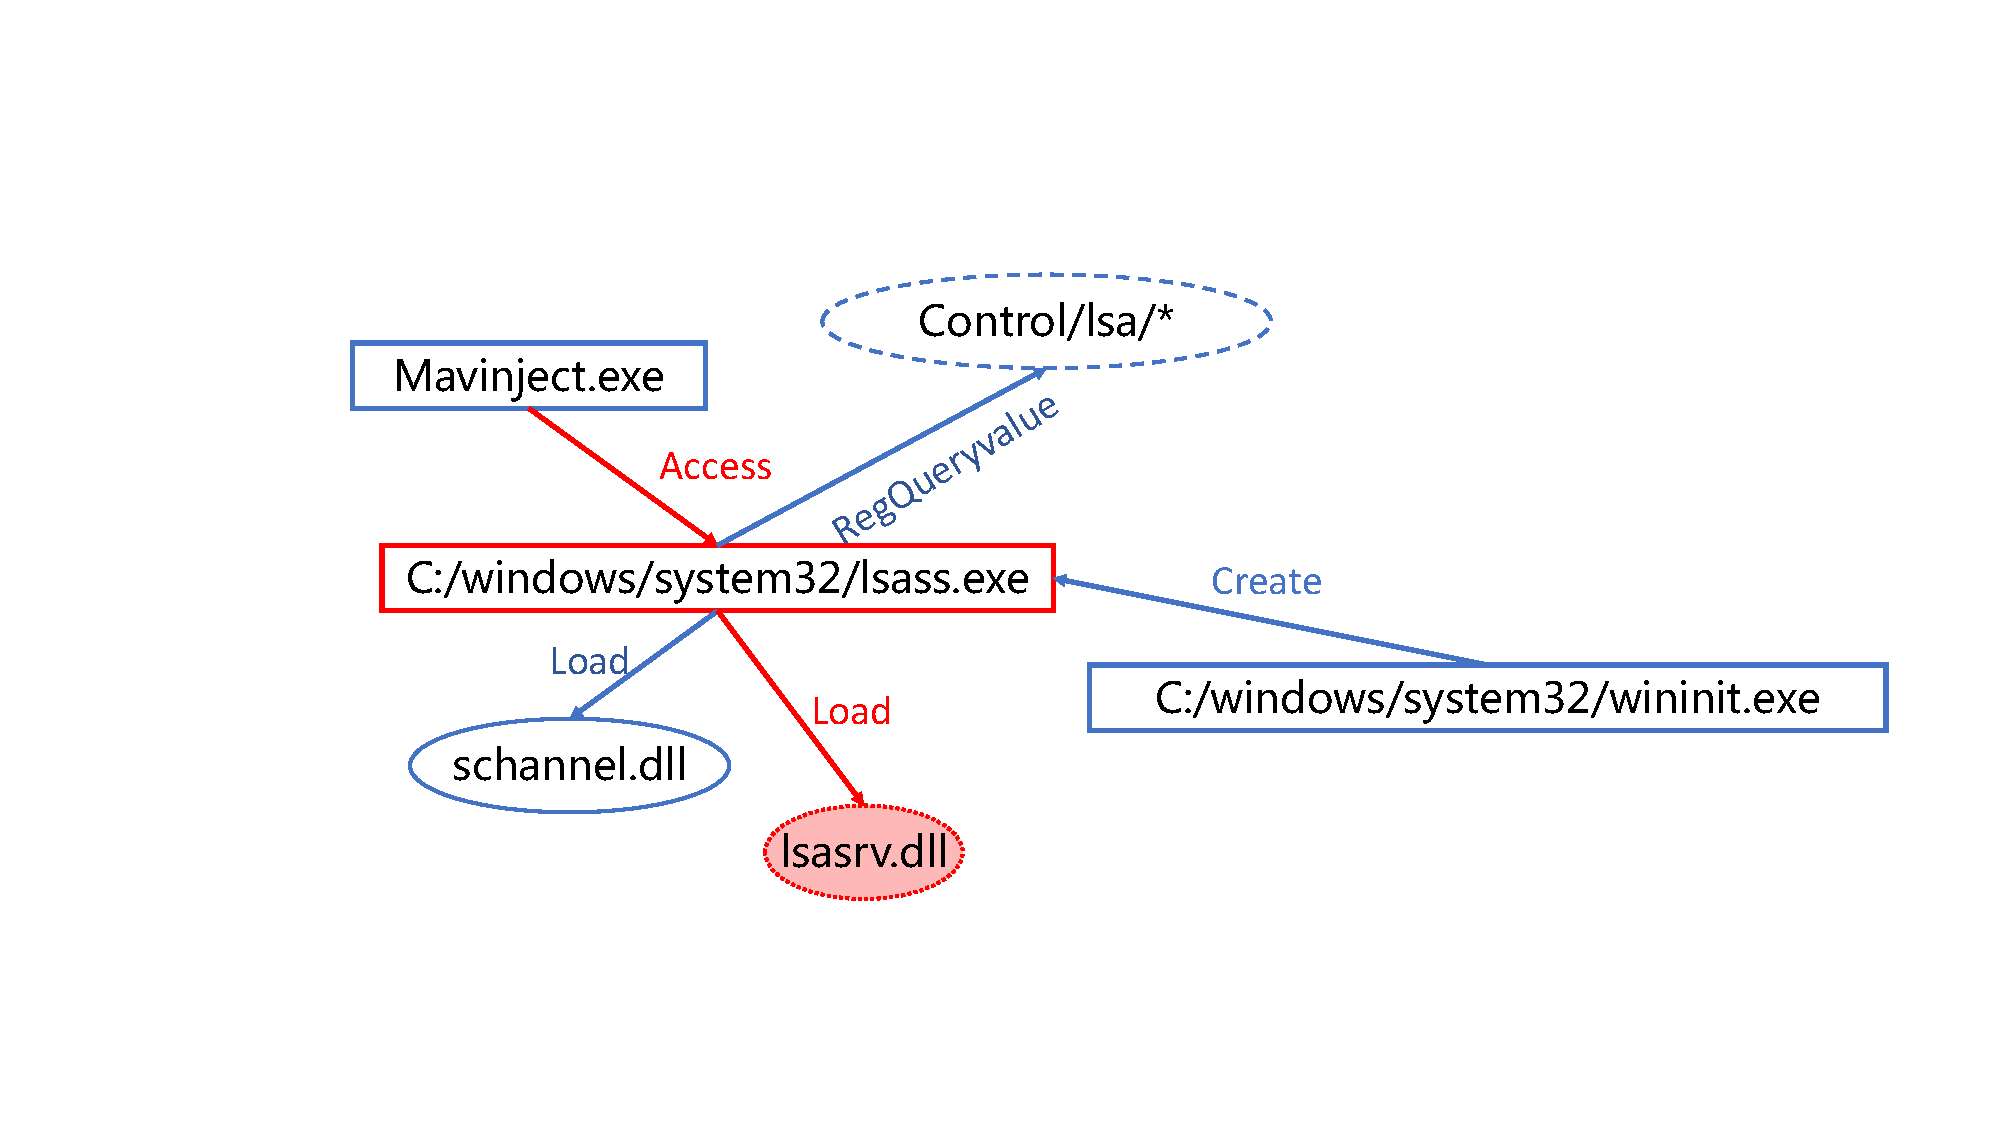
\includegraphics[width=\textwidth]{figs/process_injection.pdf}
      \caption{Process Injection}
      \label{fig:process_inj}

  \end{subfigure}

  \begin{subfigure}{.5\textwidth}
      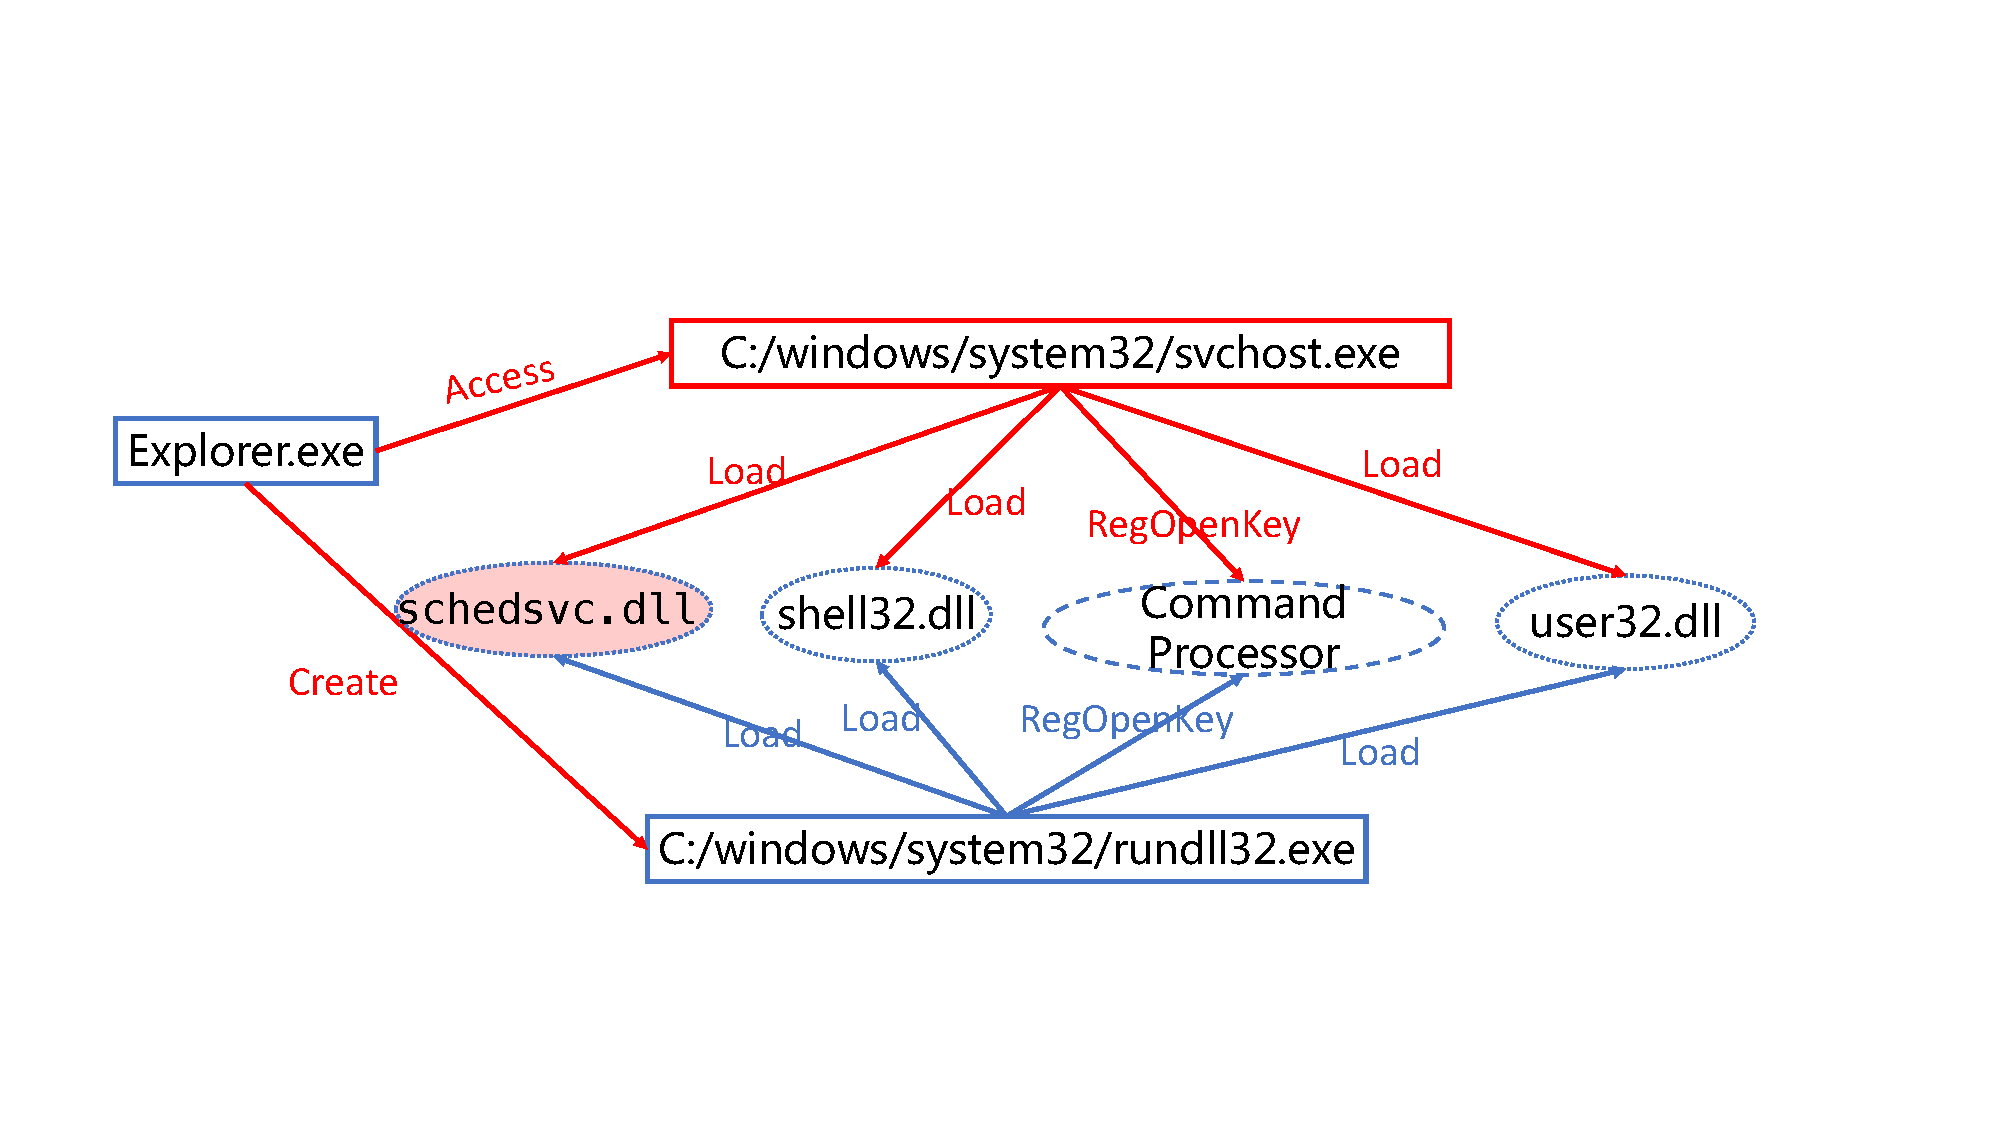
\includegraphics[width=\textwidth]{figs/Process Hollow.pdf}
      \caption{Process Hollow}
      \label{fig:hollow}

  \end{subfigure}
  \hfill
  \begin{subfigure}{.5\textwidth}
      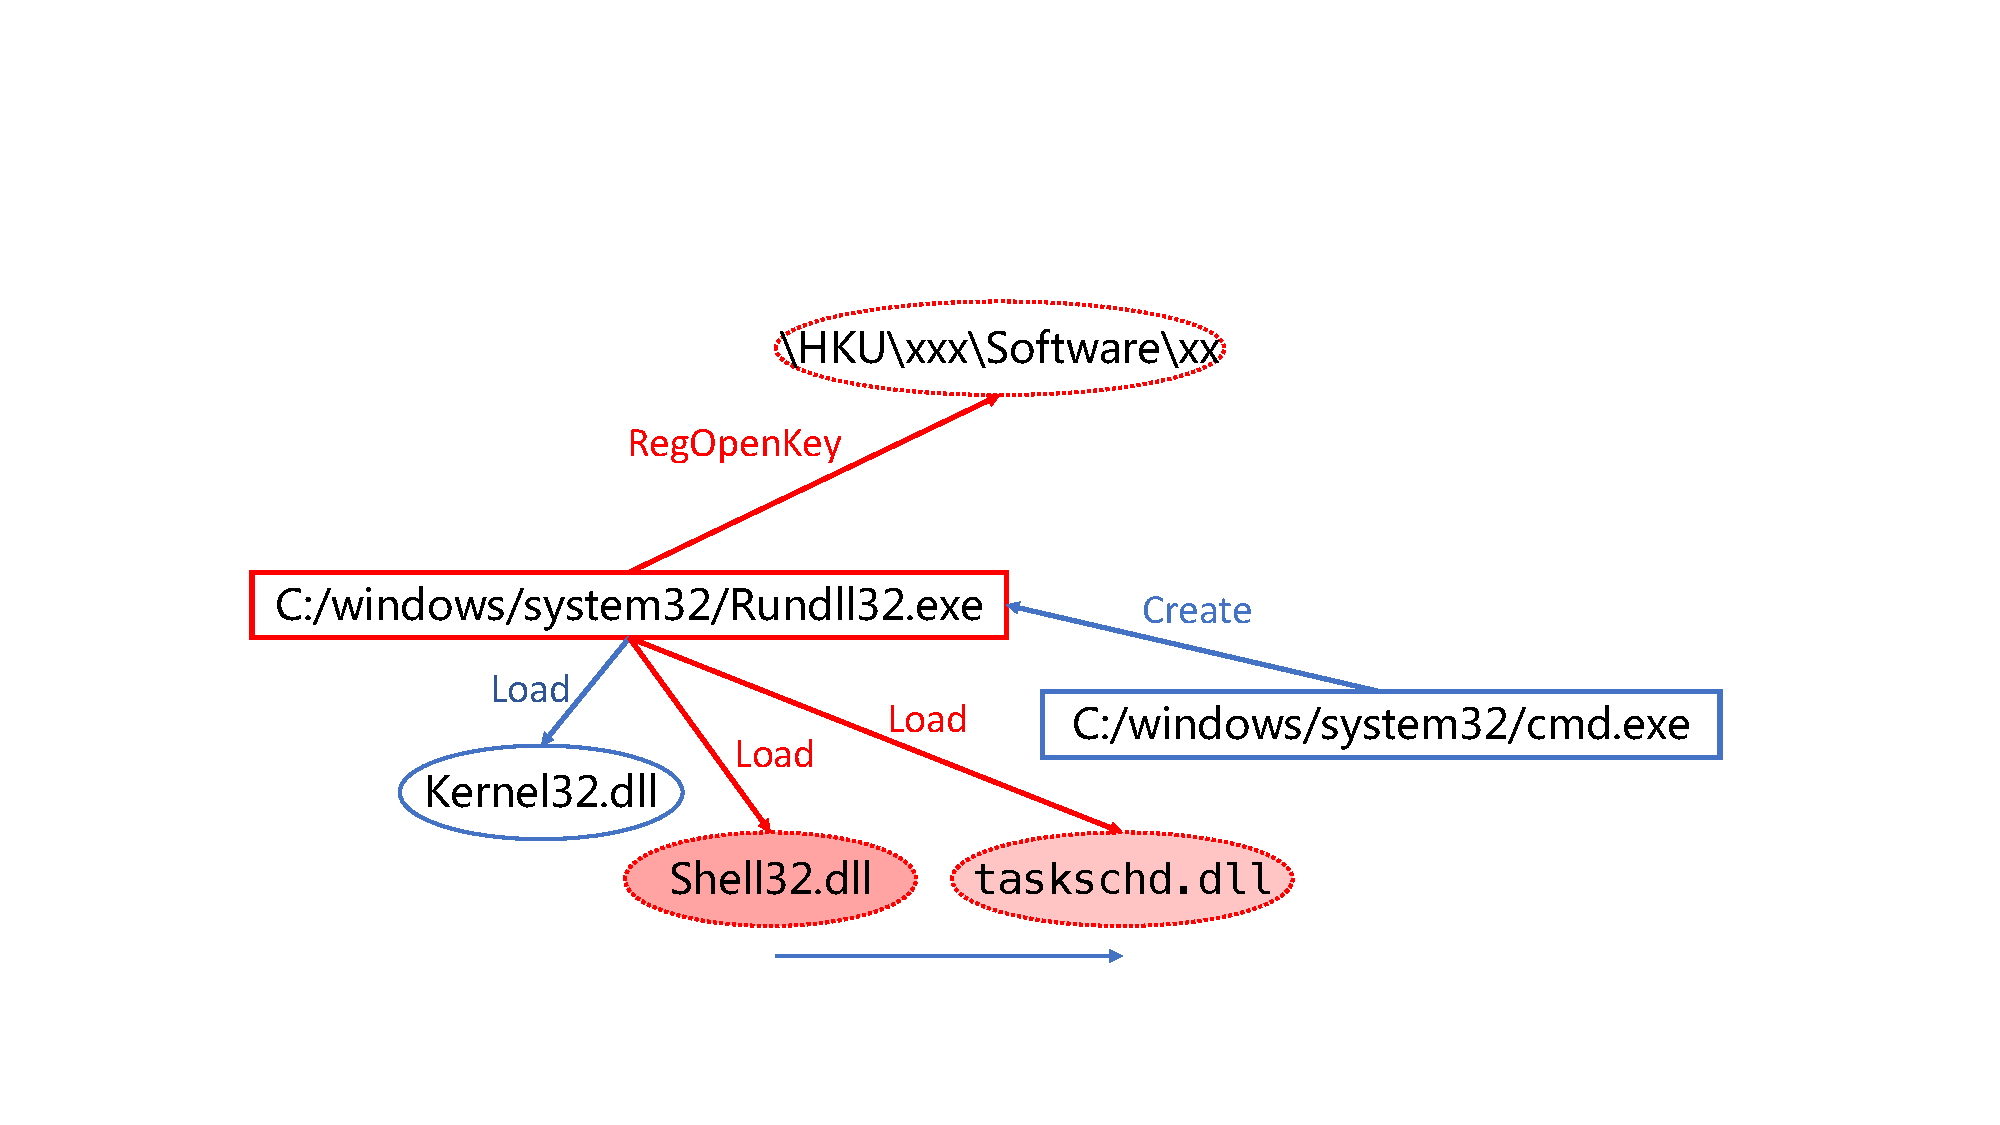
\includegraphics[width=\textwidth]{figs/Dll Side-Loading.pdf}
      \caption{Dll Side-Loading}
      \label{fig:side-load}
  \end{subfigure}

  \centering
 \caption{Each solid node in the graph represents detected signal, which has violated various constraints.}
\end{minipage}
\hfill
\begin{minipage}[b]{0.34\textwidth} 

  \begin{subfigure}{.99\textwidth}
      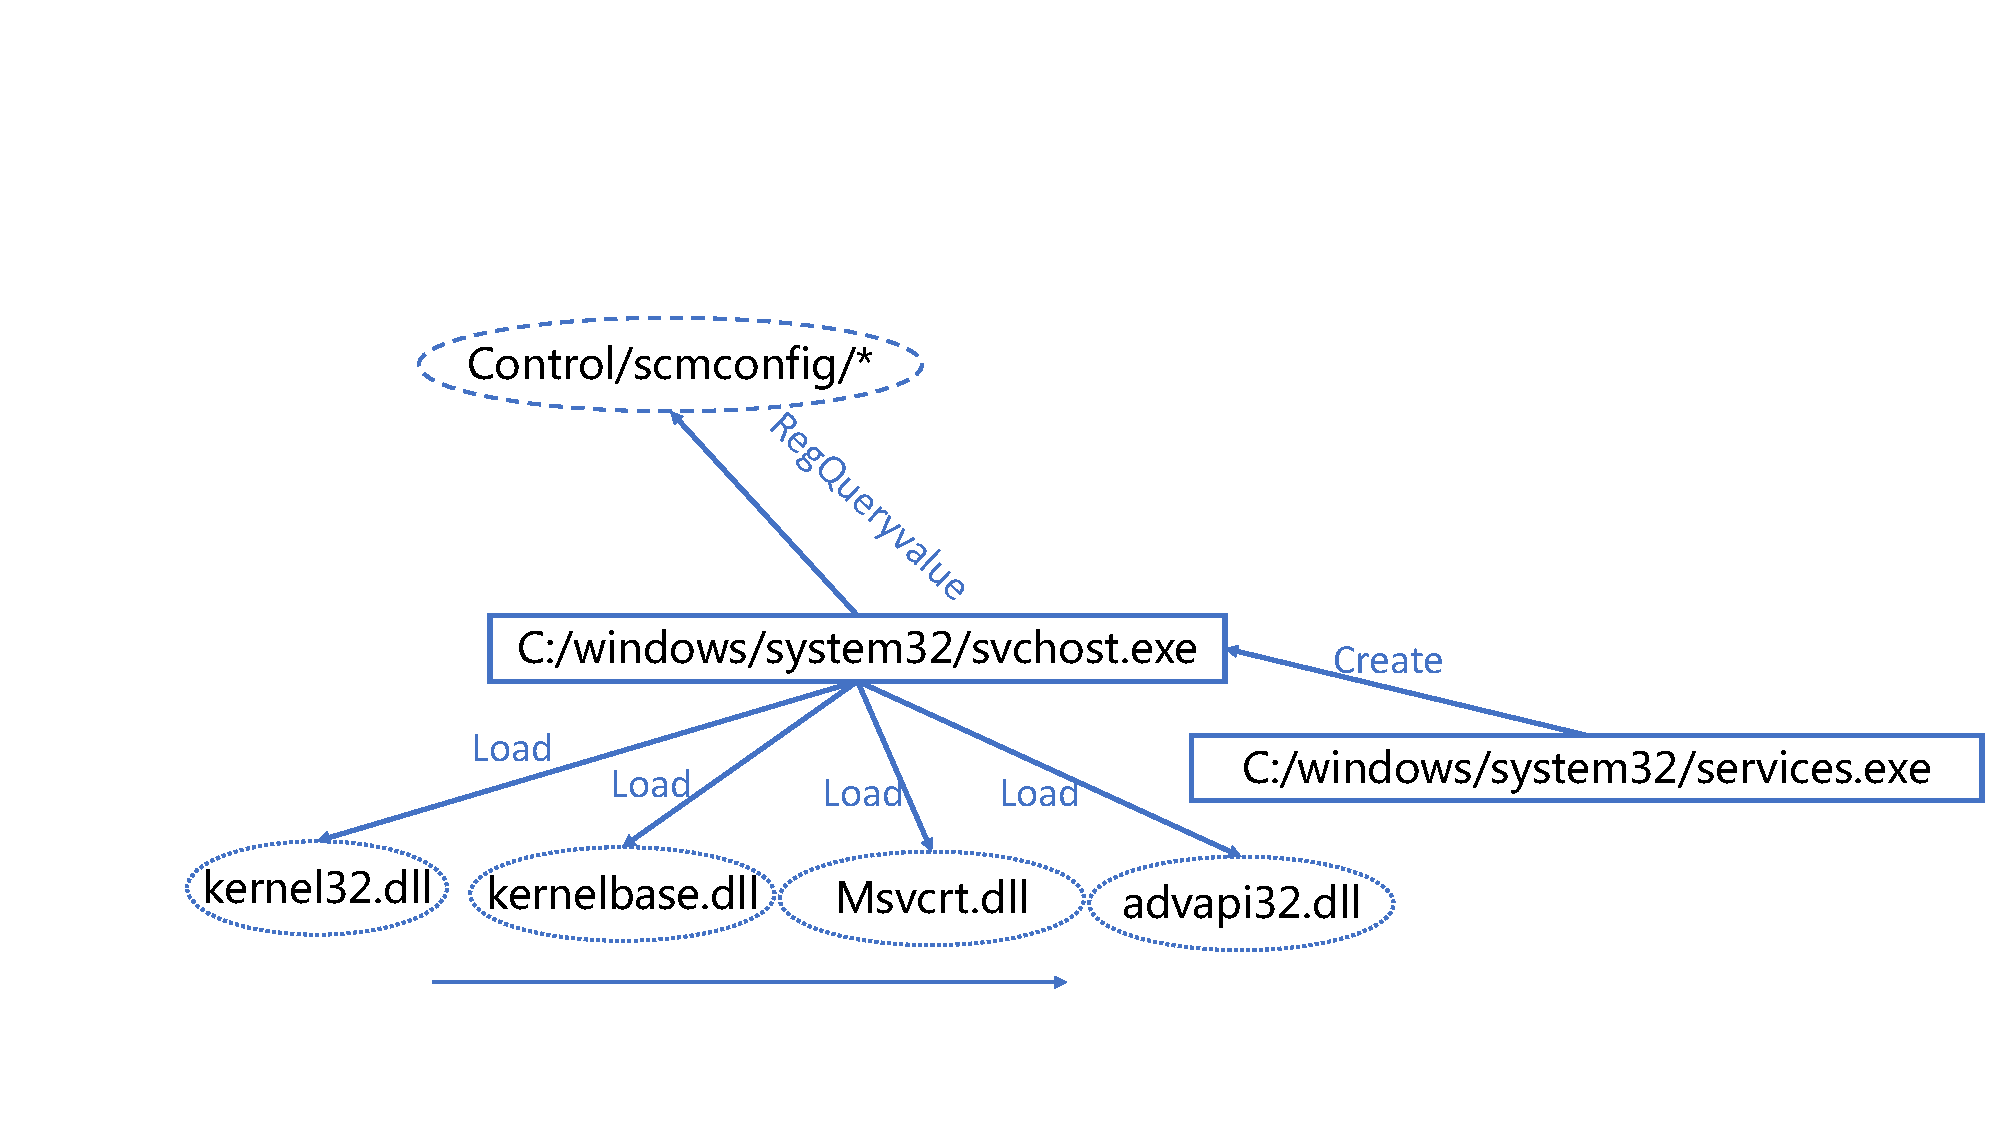
\includegraphics[width=\textwidth]{figs/svchost.pdf}
      \caption{Svchost Behavioral Invariants}
      \label{fig:svc-cons}
  \end{subfigure}
  \hfill
  \vspace{0.9cm}
  \begin{subfigure}{.99\textwidth}
      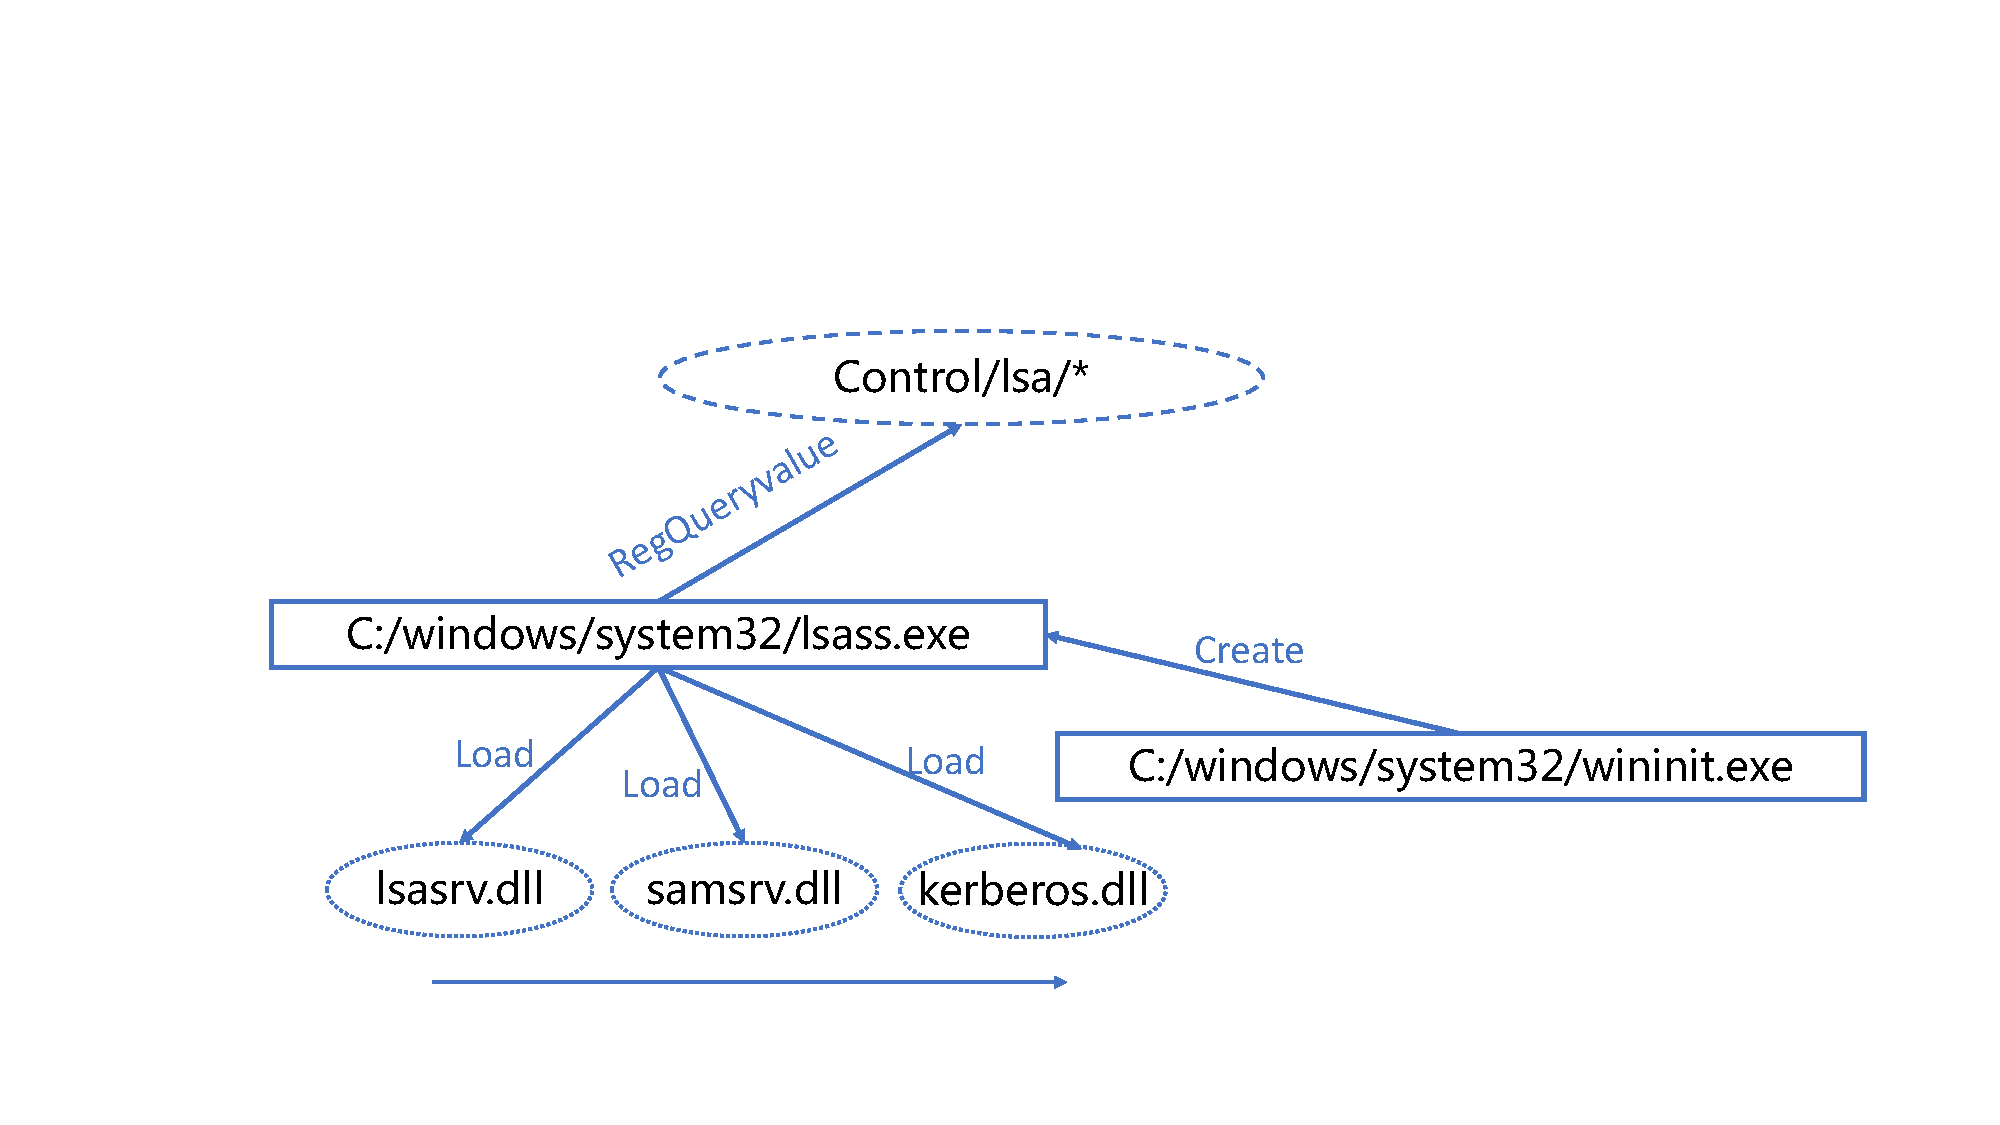
\includegraphics[width=\textwidth]{figs/lsass.pdf}
      \caption{Lsass Behavioral Invariants}
      \label{fig:lsass-cons}
  \end{subfigure}
  \vspace{-0.9cm}
\caption{Behavioral Invariants}
\label{fig-fdh}
\end{minipage}
\end{figure*}

\subsubsection{Evaluation on Attack for Various Processes}
We launched attacks on 70 system processes using 4 stealthy techniques, targeting 23 malicious functionalities. Due to space constraints, we show 10 typical malicious functions.
As illustrated in Table~\ref{table:eva-attack}, based on the 40 attacks we synthesized, our method detected 66 out of 70 processes in the worst-case scenario, thus achieving a very low false negative rate.
However, some errors still persist, which we intend to delve into further.

\begin{table*}[h!]
    \centering
    \scalebox{0.85}{
    \begin{tabularx}{\textwidth}{|X|X|X|X|X|X|X|X|X|X|X|}
        \hline
        & \textbf{BU} & \textbf{C} & \textbf{FM} & \textbf{FS} & \textbf{ST} & \textbf{PE} & \textbf{KM} & \textbf{FA} & \textbf{SE} & \textbf{E} \\
        \hline
\multicolumn{1}{|l|}{\textbf{PM}} & \multicolumn{1}{l|}{69/70}   & \multicolumn{1}{l|}{69/70}  & \multicolumn{1}{l|}{69/70}   & \multicolumn{1}{l|}{69/70}   & \multicolumn{1}{l|}{69/70}   & \multicolumn{1}{l|}{69/70}   & \multicolumn{1}{l|}{69/70}   & \multicolumn{1}{l|}{69/70}   & \multicolumn{1}{l|}{69/70}   & \multicolumn{1}{l|}{69/70}  \\ \hline
\multicolumn{1}{|l|}{\textbf{PH}} & \multicolumn{1}{l|}{69/70}   & \multicolumn{1}{l|}{67/70}  & \multicolumn{1}{l|}{67/70}   & \multicolumn{1}{l|}{68/70}   & \multicolumn{1}{l|}{68/70}   & \multicolumn{1}{l|}{69/70}   & \multicolumn{1}{l|}{67/70}   & \multicolumn{1}{l|}{67/70}   & \multicolumn{1}{l|}{69/70}   & \multicolumn{1}{l|}{70/70}  \\ \hline
\multicolumn{1}{|l|}{\textbf{PI}} & \multicolumn{1}{l|}{66/70}   & \multicolumn{1}{l|}{65/70}  & \multicolumn{1}{l|}{67/70}   & \multicolumn{1}{l|}{69/70}   & \multicolumn{1}{l|}{67/70}   & \multicolumn{1}{l|}{68/70}   & \multicolumn{1}{l|}{69/70}   & \multicolumn{1}{l|}{67/70}   & \multicolumn{1}{l|}{67/70}   & \multicolumn{1}{l|}{68/70}  \\ \hline
\textbf{DLL}                      & 69/70                        & 68/70                       & 67/70                        & 67/70                        & 69/70                        & 66/70                        & 67/70                        & 67/70                        & 68/70                        & 66/70                       \\ 
        \hline
    \end{tabularx}}
    % \caption{Detection of Process Count for Various Techniques and Malicious Activities}
    \caption{Detection of Process Count for Various Techniques and Malicious Activities, where BU is short for BypassUAC, C for Compression, FM for File Monitor, FS for File Scan, ST for Scheduled Task, PE for Privilege Escalation, KM for Keyboard Monitor, FA for Forced Authentication, SE for Service Execution, E for Exfiltration, PM for Process Masquerade, PH for Process Hollow, PI for Process Injection, and DLL for DLL Side-Loading.}
    % \smallskip
    % \small \textit{Abbreviations: BU - BypassUAC, C - Compression, FM - File Monitor, FS - File Scan, ST - Scheduled Task, PE - Privilege Escalation, KM - Keyboard Monitor, FA - Forced Authentication, SE - Service Execution, E - Exfiltration, PM - Process Masquerade, PH - Process Hollow, PI - Process Injection, DLL - DLL Side-Loading}
    \label{table:eva-attack}
\end{table*}

% \smallskip
% \noindent
\paragraph{Analysis of False Negatives.}
We discovered two primary reasons for these errors after thoroughly examining the incorrect cases:


\textit{Insufficient Knowledge for Certain Processes}:  The internal knowledge of the LLMs is limited for some processes. Consider the process \textit{amdfendrsr.exe}, which is a core system process associated with AMD Crash Defender Service. However existing knowledge base lacks comprehensive details on this process. Consequently, the constructed profile results in weak Behavioral Invariants, which render the model incapable of detecting attacks that violate the \textit{amdfendrsr.exe} process Behavioral Invariants.

\textit{Some stealthy attack does not violate any Behavioral Invariants}: There are some stealthy attacks that do not violate any established Behavioral Invariants. For example, it is possible to inject a DLL into a process that cannot load it natively. A \textit{lsasrv.dll} would not be loaded naturally by \textit{svchost.exe} if a malicious DLL named \textit{lsasrv.dll} was injected into it, so no DLL constraints would be validated. Another example is that some \textit{rundll32.exe} attacks operate within their legitimate bounds. For instance, Live-off-the-land\cite{barr2021survivalism} attacks leverage the normal functionality of legitimate programs for malicious purposes.




\subsubsection{Evaluation on Normal Workloads}
As previously mentioned, the GitHub project \cite{evtx-baseline2022} provides logs for different Windows versions specifically Windows 7, Windows 10, and Windows 11. We utilized these logs to assess the false positive rate (i.e., false alarms) of our method in these scenarios.
As illustrated in Figure~\ref{fig-eva-normal}, in the Windows 10 system, our method had 1 false positive out of 47 processes in our list. In Windows 11, there were 3 false positives out of 52 processes, and in Windows 7, the performance was the poorest with 2 false positives out of 13 processes.

\begin{figure}[h]
    \centering
      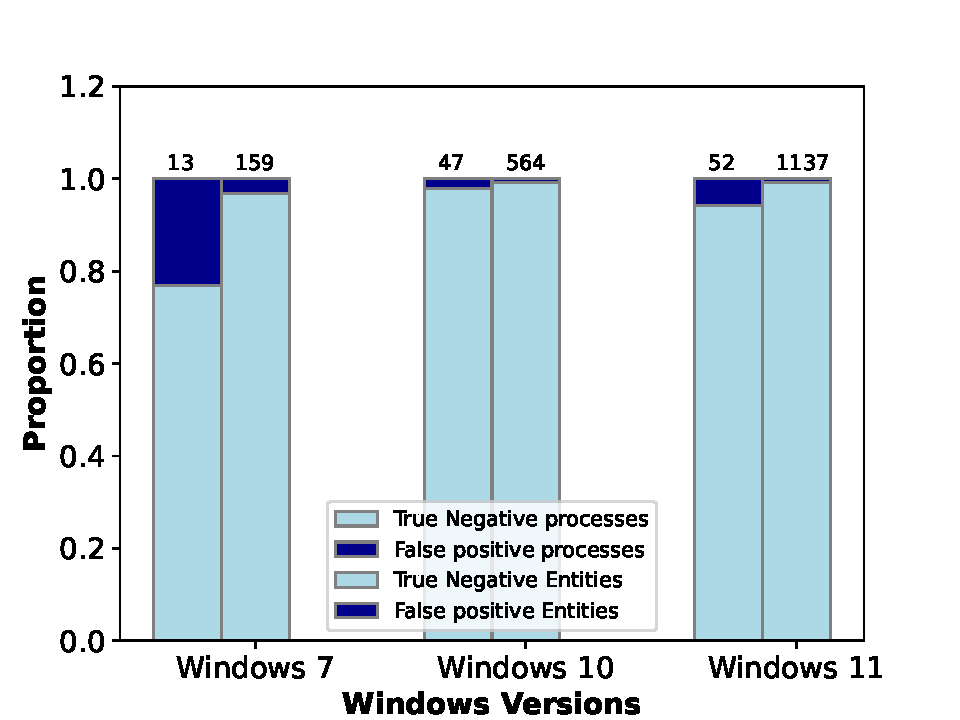
\includegraphics[width=0.45\textwidth]{figs/normal_chart.pdf}
    \caption{Evaluation on Normal Workloads.}
    \label{fig-eva-normal}
\end{figure}

\smallskip
\paragraph{Analysis of False Positives.}
After a detailed analysis of the various causes of false positives, we identified the following key issues:

\textit{Uniformity in LLM's Results}: The LLM system tends to offer overly single results. For instance, the parent processes of \\ \textit{C:/Windows/explorer.exe} can vary widely, including options like \textit{C:/Windows/explorer.exe} itself and \textit{C:/Windows/System32/userinit.exe}. However, LLMs only provide feedback for \textit{userinit.exe}. This means that any normal process not having \textit{userinit.exe} as its parent process gets flagged incorrectly. This issue is also evident in processes like \textit{dllhost.exe} and \textit{conhost.exe} which can have multiple parent processes.

\textit{Overconfidence in LLM's Analysis}: For some events that might be absent in a few scenarios, the LLM tends to be overly confident. A case in point is the event \\ \textit{<lsass.exe RegSetValue,hklm/system/currentcontrolset/control/lsa/*>}. 
While this event is expected to occur in the majority of scenarios, there are specific situations where it might not manifest.  Another example includes a set of three events:  \textit{<lsass.exe,Load,lsasrv.dll>-><lsass.exe,Load,samsrv.dll>-><lsass.exe,Load,kerberos.dll>)}. Typically, these events appear together. However, the event associated with kerberos.dll can sometimes be absent or loaded ahead of time. Consequently, having a stringent expectation for normal programs to execute in a specific order leads to false alarms.

\textit{Operating System Version Discrepancies}: Our process profile was built based on Windows 10 scenarios. As a result, while false positives are lower in a Windows 10 environment, they're notably higher for Windows 7. This is because Windows 10, being a newer version compared to Windows 7, has undergone changes in process behavior. For instance, in Windows 7, a single \textit{svchost.exe} might host multiple services. In contrast, in Windows 10, it can only host one. Consequently, profiles constructed for Windows 10 tend to have higher false positives when applied to Windows 7.



\subsubsection{Evaluation on Simulated APT scenarios}
We construct 10 simulated trojan-based APT attack scenarios by combining single attack behavior and compare our method against three state-of-the-art techniques. 

\begin{itemize}
    \item \textbf{ThreaTrace}\cite{wang2022threatrace} constructs a unique model for each type of node within a provenance graph aiming to identify anomalies at the node level. Since this is a method based on anomalous nodes, we can compare the final false positive and false negative rates fairly.
    \item \textbf{ATLAS}\cite{alsaheel2021atlas} uses graphs to derive attack and non-attack sequences, as well as sequence models to discern attack patterns. we compared the detection effect at the node level because our method is process-centered.
    \item \textbf{Shadewatcher} \cite{zengy2022shadewatcher} have adapted the method originally designed for information flow for our comparative analysis. First, we use Shadewatcher's embedding method to get the node's vector, as soon as the embedding of the node is obtained, we use LOF anomaly detection to determine the detection rate of abnormal nodes.
\end{itemize}

\begin{table}
    \centering
    \small 
    \scalebox{0.85}{
    \begin{tabular}{|c|c|c|c|c|}
        \hline
        \multicolumn{1}{|c|}{Attack ID} & \multicolumn{2}{c|}{Process} & \multicolumn{2}{c|}{Entity} \\
        \cline{2-5}
        & \#Attack & \#Non-attack & \#Attack & \#Non-attack \\
        \hline
        S-1 & 8 & 738 & 41 & 2286 \\
        S-2 & 8 & 939 & 41 & 2669 \\
        S-3 & 9 & 1003 & 43 & 2704 \\
        S-4 & 7 & 713 & 18 & 2051 \\
        S-5 & 9 & 1134 & 45 & 3038 \\
        S-6 & 7 & 893 & 38 & 2277 \\
        S-7 & 8 & 718 & 21 & 2101 \\
        S-8 & 8 & 1092 & 42 & 2951 \\
        S-9 & 8 & 1090 & 42 & 2699 \\
        S-10 & 7 & 748 & 21 & 2157 \\
        Avg. & 8 & 907 & 35 & 2493 \\
        \hline
    \end{tabular}}
    \caption{Process-based and entity-based investigation results.}
\end{table}

\begin{table}[ht]
\scalebox{0.85}{
\centering
\begin{tabular}{|l|c|c|c|c|}
\hline
\textbf{Method} & \textbf{P(Avg.)} & \textbf{R(Avg.)} & \textbf{F1(Avg.)} \\
\hline
ThreaTrace & 1.01\% & 35.84\% & 2.00\%  \\
ATLAS & 9.63\% & 57.83\% & 14.68\%\\
Shadewatcher & 6.52\% & 6.20\% & 6.41\%  \\
\textit{\tool} (ours) & 96.25\% & 90.15\% & 92.79\%  \\
\hline
\end{tabular}}
\caption{Comparison of different methods.}
\label{tab:comparison}
\end{table}

The table that \tool is effective in reporting trojan-based APT attack (with a precision of 96.25\% and a recall of 90.15\%), at the cost of minimum runtime overhead (of on average 2.3s), much better than other methods.
In the following examples, we will explain why our method works, but other methods fail to recognize or misidentify.
\paragraph{Case1: Process Masquerade:} Process Masquerade imposes constraints on \textit{svchost.exe}, as illustrated in Figure~\ref{fig:process_mas}. As a result of our method, we can observe that \textit{svchost.exe} normally executes in the path \textit{C:/windows/system32/svchost.exe}, with \textit{services.exe} as its parent process. Malicious \textit{svchost.exe} violates both execution path and parent process constraints in this example, resulting in its classification as malicious. Current methods \cite{wang2022threatrace} are effective to detect attacks that manifest significant behavioral changes in files and networks, such as compression, file scanning, and exfiltration, using graph structures. It is however difficult to identify attacks with these graph-structured methods, such as service execution, and forced authentication, that do not introduce obvious changes to the graph. 

\paragraph{Case2: Process Injection:} As illustrated in the Figure~\ref{fig:process_inj}, the attacker injects a malicious \textit{lsasrv.dll} into the \textit{lsass.exe} process. However, a normal \textit{lsass.exe} process follows a specific load chain where \textit{lsasrv.dll} is definitely followed by the loading of \textit{samsrv.dll}. The violation of these temporal constraints indicates malicious activity. No specific information is available regarding the DLL. Current methods\cite{wang2022threatrace} are unable to distinguish between attacks and non-attacks based on the graphical structure, making detection impossible.

\paragraph{Case3: Process Hollow:} Shadewatcher\cite{zengy2022shadewatcher} is designed to embed itself into every node. In a process hollowing attack as shown in Figure~\ref{fig:hollow}, the depicted \textit{svchost.exe} is hollowed out and the memory functionalities of \textit{cmd.exe} are injected into it. As a result, \textit{svchost.exe} and \textit{cmd.exe} manifest similar functionalities. If we employ Shadewatcher's method of embedding, both \textit{cmd.exe} and \textit{svchost.exe} will have comparable embeddings. Since \textit{cmd.exe} exhibits normal behavior, it becomes indistinguishable whether the behavior of \textit{svchost.exe} is malicious or not. This inability to differentiate results in the failure to detect the attack.

\paragraph{Case4: Dll side-Loading:} Similar to process injection, DLL Side-Loading also violates the normal load chain, indicating an aberration from the standard operating procedure, and thereby suggesting malicious activity. According to current methods\cite{wang2022threatrace}, the graphical structure cannot distinguish attacks from non-attacks, making detection impossible.




\subsection{Efficiency}
\label{sec-eff}
Regarding the efficiency concerns of our system, we aim to investigate the following questions:
1) How long does it take for our method to construct a profile for each process?
2) Which step in the process profile creation is the most time-consuming?
To determine this, we have divided the process profile construction into five steps. We then individually measure the runtime and costs for each step, as illustrated in Table~\ref{tab:process_metrics}.
In our study, we found that the process behavior tree construction is the most time-consuming and expensive part of the project. It takes 21 minutes and \$3.51 to build a profile for a single process.

\begin{table}[h!]
    \centering
    \scalebox{0.85}{
    \begin{tabular}{|l|c|c|}
        \hline
        & Running Time & Cost \\
        \hline
        Behavior Tree Construction & 501(s) & 1.23\$ \\
        \hline
        Command Generate & 156(s) & 0.85\$ \\
        \hline
        Command Execution & 200(s) & 0\$ \\
        \hline
        Constraint Extraction & 201(s) & 0.51\$ \\
        \hline
        Validation & 321(s) & 0.92\$ \\
        \hline
        Total & 1379(s) & 3.51\$ \\
        \hline
    \end{tabular}}
    \caption{Running Time and Cost for various processes}
    \label{tab:process_metrics}
\end{table}

\subsection{Ablation Study}
\label{sec-ab-study}
An ablation study was conducted integrating data from 10 different attack scenarios with three normal scenarios as shown in ~\ref{fig:comparison}. In total, the attack scenarios included 70 attack processes, while the normal scenarios comprised 1960 regular processes.
The ablation study aims at assessing the effectiveness of the divergent and validation methods that are integral to \tool's performance. 
This experiment modified the approach by either removing one or both of these steps.
1) \textbf{\tool-NO-Tree-Construction}: The Process Tree Construction Module is deactivated. This means all data is input directly into the system without any hierarchical structuring.
2) \textbf{\tool-NO-Validation}: The Validation Module is inactive, which means that real log validation and multi-round session debate validation have been disabled.
3) \textbf{\tool-NO-All}: This indicates that the process tree Construction and validation steps have both been removed.

\begin{figure}[h]
    \centering
    \begin{subfigure}[b]{0.23\textwidth}
        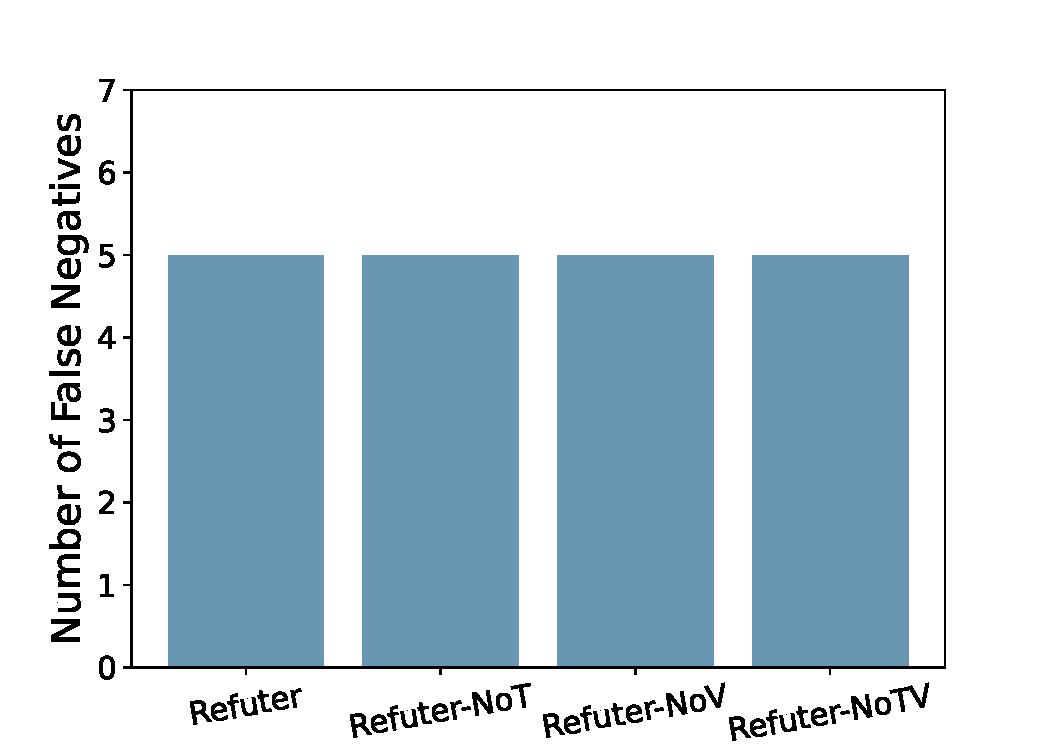
\includegraphics[width=\textwidth]{figs/FN.pdf}
        \caption{False Negative for In Attack Scenario}
        \label{fig:missed_attacks}
    \end{subfigure}
    \hfill
    \begin{subfigure}[b]{0.23\textwidth}
        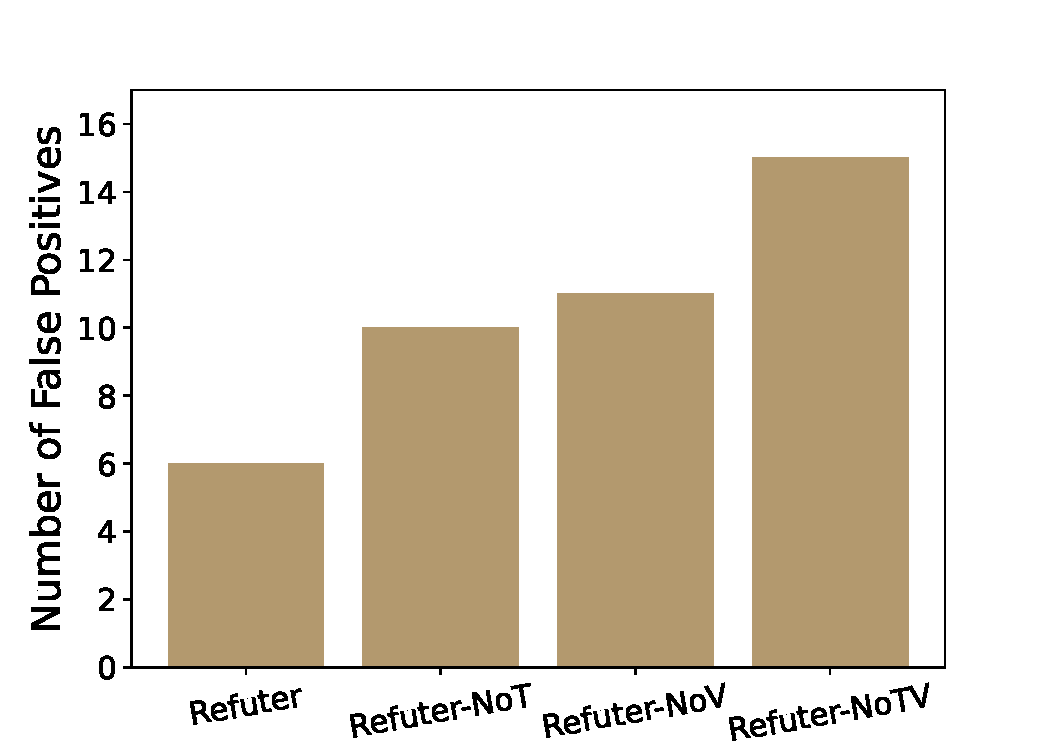
\includegraphics[width=\textwidth]{figs/FP.pdf}
        \caption{False Positive for Normal Scenario}
        \label{fig:false_positives}
    \end{subfigure}
    \caption{Comparison of different methods in terms of False Negative and false positives}
    \label{fig:comparison}
\end{figure}
We found no significant difference in attack scenarios between our method and the control method. Our approach, however, achieved the lowest false positive rate for normal scenarios.
In the following, examples are used to illustrate the role of adding behavior trees and validation links in reducing false positives.
Without the construction of the behavior tree, we obtain many constraints that are too broad.
For example, the behaviors that we mind and that \textit{svchost.exe} must obey when hosting certain services, like \textit{PhoneSvc} and \textit{NgcSvc}, must have behavior \textit{svchost.exe,CreateFile,*/localservice/appdata*}. However, for other services like the \textit{DHCP service}, this behavior isn't necessarily required. These are not behaviors that all processes must adhere to, resulting in a high false positive rate when tested normally. 

We aim to demonstrate the effectiveness of our cross-session validation approach. From our experiments, it's evident that for actions that are undeniably factual, the three agents can reach a consensus after multiple rounds of debate. For instance, \textit{lsass.exe} will unquestionably load \textit{c:/windows/system32/lsasrv.dll}. On the other hand, for behaviors that aren't necessarily factual, the agents diverge in their opinions after several debate rounds and pinpoint the underlying reasons. For example, the behavior of \textit{sass.exe} with \textit{RegSetValue, hklm/system/currentcontrolset/control/lsa/} is not mandatory.



\subsection{Explanation Validation}
\label{sec-explanation-val}
To confirm the accuracy of the behavioral invariant we extracted, we searched Google, blogs, books, etc. In some public reports, we found consistency between their findings and our constraints.

There are some crucial documents\cite{nasbench}, including a technical document that outlines 15 essential system processes and their execution paths. For instance, in the case of \textit{lsass.exe}, the document indicates that its parent process is \textit{wininit.exe}, it does not have a fixed child process, and its execution path is \textit{c:/windows/system32/lsass.exe}. It aligns with the knowledge we have gained through LLMs.
There is also document\cite{windows10dll} about static call relationships between Windows DLLs. \textit{Lsass.exe} will undoubtedly load \textit{lsasrv.dll}, and \textit{lsasrv.dll} and \textit{samsrv.dll} have a static link relationship. This knowledge also remains consistent with what we have learned through LLMs.

% https://nasbench.medium.com/windows-system-processes-an-overview-for-blue-teams-42fa7a617920

% https://windows10dll.nirsoft.net/lsasrv_dll.html

\begin{table*}
    \centering
    \scalebox{0.85}{
    \begin{tabular}{|l|l|l|p{6cm}|}
        \hline
        Masquerading Type & Malware/APT & Targeting process & Description \\
        \hline
        \multirow{2}{*}{Process Masquerading}
        & GALLIUM\cite{cybereason2023} & \textit{cmd.exe} & Attackers use a renamed \textit{cmd.exe} file to evade detection \\
        \cline{2-4}
        & DCSrv\cite{checkpoint2021} & \textit{svchost.exe} & Attackers masquerade as a legitimate \textit{svchost.exe} process to encrypt all computer volumes \\
        \cline{2-4}
        & APT29\cite{mitre_g0016} & \textit{svchost.exe/rar.exe} & Attackers rename benign processes for use in various stages of the attack \\
        \hline
        \multirow{3}{*}{Dynamic-link Library Injection} & Aria-body\cite{checkpoint2020} & \textit{rundll32.exe/dllhost.exe} & Aria-body loader injects itself to another process \\
        \cline{2-4}
        & BlackEnergy\cite{fsecure2019} & \textit{svchost.exe} & The driver component injects the main DLL component into \textit{svchost.exe} \\
        \cline{2-4}
        & Sykipot\cite{att2023} & \textit{outlook/iexplore.exe} & The malware scans running processes for outlook or iexplore and injects a DLL \\
        \hline
        \multirow{2}{*}{Process Hollowing} & RCSession\cite{secureworks} & \textit{svchost.exe} & RCSession was launched from \textit{English.rtf} via a hollowed \textit{svchost.exe} \\
        \hline
        \multirow{2}{*}{Dll side-Loading} & APT3\cite{mitre_g0022} & \textit{Chrome.exe} & Attackers side load DLLs with a valid version of Chrome with their tools \\
        \cline{2-4}
        & APT29\cite{mitre_g0016} & \textit{Msoev.exe} & Attackers use an HTA file to drop three executables into the \%TEMP\% directory \\
        \hline
    \end{tabular}}
    \caption{Real world APT Attack using stealthy technical}
    \label{tab:real_world}
\end{table*}

\subsection{Real-world Validation}
\label{sec-real-world}

We collected some publicly available malicious software related to APTs, as shown in Figure~\ref{tab:real_world}.
Using this real-world data, we wanted to validate the effectiveness of our method. As a result, we can detect most types of stealthy attacks using our method, including these four types of trojan stealthy attacks.
We reviewed a total of 11 real APT attack reports and analyzed the data. Finally, we found that 9 out of 11 attacks could be detected by our method.

Evaluation on the DARPA-TC dataset demonstrates that our method can identify stealthy attacks.

Here are three specific examples.
\noindent
{\bf APT29 \cite{mitre_g0016}.}
We have analyzed malicious payloads associated with APT29, specifically focusing on \textit{python.exe}. According to the profile we constructed for a typical Python application, \textit{python.exe} would certainly load \textit{pythonxx.dll} and \textit{vcruntime140.dll}. However, in the dataset related to the malicious \textit{python.exe} used by APT29, we didn't find evidence of these two DLLs being loaded. This suggests that the \textit{python.exe} under scrutiny is likely not a standard or legitimate version.

\noindent
{\bf DCSrv\cite{checkpoint2021}.}
Moving on to the malware named DCSrv, we located this malicious software in the VirusTotal sandbox. We observed that it masquerades as \textit{svvhost.exe} with an execution path of \\ \textit{C:/Users/user/Desktop/svvhost.exe}. \textit{Svchost.exe} has been obfuscated through string obfuscation, and its execution path is different from the typical \textit{svchost.exe} path.

\noindent
{\bf Sykipot\cite{att2023}.}
It appears that the malicious program Sykipot launches process injection attacks against \textit{firefox.exe}. The injected malicious dll is named \textit{wship4.dll}. There is no legitimate DLL by this name, but we did find \textit{wship6.dll}, which is related to IPv6 network operations. In order for \textit{wship6.dll} to interact correctly, \textit{WS2\_32.dll} must also be loaded. Furthermore, there was no indication that \textit{WS2\_32.dll} was loaded, indicating malicious activity.












\section{Related work}

% \paragraph{Stealthy APT Attacks}
% Advanced Persistent Threats (APTs) are sophisticated, targeted, evolving, and steathy cyberattacks launched by specialized groups against high-risk entities, such as nuclear power plants, banks, and governments. APTs are using stealthy tactics such as name obfuscation\cite{cybereason2023,checkpoint2021,intrinsec}, process injection\cite{checkpoint2020,fsecure2019}, process hollow\cite{secureworks}, side-loading DLLs\cite{mitre_g0022,mitre_g0016}, and manipulating legitimate system utilities in order to bypass traditional security defenses due to the dynamic cyber threat landscape\cite{barr2021survivalism}. An example is Process injection, a popular technique for enabling malicious code to run within another process's address space.  Additionally, attackers use tools like \textit{rundll32.exe} to execute benign binaries and \textit{powershell.exe} to launch script-driven attacks\cite{li2019effective}. By exploiting these widely recognized and trusted tools, adversaries can discreetly penetrate and control their target systems.

% \paragraph{Provenance Graph-Based APT Detection}
% Chenyan  usenix chair
% Threat Detection and Investigation with System-level Provenance Graphs: A Survey
% CONAN: A Practical Real-time APT Detection System with High Accuracy and Efficiency
% Effective and Light-Weight Deobfuscation and Semantic-Aware Attack Detection for PowerShell Scripts
% AttacKG: Constructing Technique Knowledge Graph from Cyber Threat Intelligence Reports
% RATScope: Recording and Reconstructing Missing RAT Attacks for Forensic Analysis with Semantics on Windows
% CONAN: A Practical Real-time APT Detection System with High Accuracy and Efficiency

% PC member
% Kangkook Jee
% You Are What You Do: Hunting Stealthy Malware via Data Provenance Analysis

% Ivan Martinovic
% Survivalism: Systematic Analysis of Windows Malware Living-Off-The-Land

% Z. Berkay Celik
% ATLAS: A Sequence-based Learning Approach for Attack Investigation

% Xiapu Luo
% D IST D ET: A Cost-Effective Distributed Cyber Threat Detection System

% Adil Ahmad
% Rethinking System Audit Architectures for High Event Coverage and Synchronous Log Availability
In this section, we discuss the related work to anomaly-based detection methods. Given the expansive body of literature regarding this topic, we will only discuss the most prominent ones therein, i.e., provenance graph-based approaches, which encapsulate two main detection strategies: learning-based detection and rule-based detection.

% Provenance graph-based methods are becoming increasingly popular in detecting stealthy APT attacks, due to their ability to identify a variety of host-based threats. There are three main detection methods based on Provenance graphs: learning-based detection, and rule-based detection.

% \paragraph{Learning-based Detection}
\smallskip
\noindent
{\bf Learning-based Detection.}
Such methods initially learn a model w.r.t. provenance graphs and then conduct anomaly detection on that. Based on the learning granularity of information derived from the graph, we broadly classify the existing learning-based approaches into three categories: (1) graph-based, (2) path-based, and (3) node-based.

% require extensive training datasets and are computationally intensive. For the learning-based detection methods, we broadly classify the existing approaches into three categories : (1) graph-based, (2) path-based, and (3) node-based. %, and (5) knowledge graph embedding-based.

% The first class of detection techniques train models on benign behaviors, identifying deviations as potential cyber-attacks \yd{Add refs}. Although these methods can detect threats with impressive accuracy by integrating audit record semantics into threat analysis, existing learning solutions often fail to provide insightful and explicable results, compromising the practical utility.
% 

For the first class of approaches,
% requires extensive training datasets and is computationally intensive. 
researchers embed provenance graphs into vector space and developed tools such as StreamSpot \cite{manzoor2016fast} and Unicorn \cite{han2020unicorn} to analyze information flow graphs. Despite Unicorn's superior performance due to its thorough graph analysis, both methods face challenges in detecting stealthy threats due to graph kernel limitations. In the same way, IPG \cite{li2021hierarchical} and ProGrapher \cite{yang2023prographer} use graph-level approaches, but struggle with similar issues as StreamSpot and Unicorn. Despite the fact that many systems attempt to use data provenance for threat detection, methods that combine scope and timeliness are needed. The remarkable capabilities of KAIROS \cite{cheng2023kairos} make it an excellent competitor.

% \noindent
% {\bf Graph-based Methods.} Graph-based anomaly detection requires extensive training datasets and is computationally intensive. Researchers have embedded provenance graphs into vector space and developed tools such as StreamSpot \cite{manzoor2016fast} and Unicorn \cite{han2020unicorn} to analyze information flow graphs. Despite Unicorn's superior performance due to its thorough graph analysis, both methods face challenges in detecting stealthy threats due to graph kernel limitations. In the same way, IPG \cite{li2021hierarchical} and ProGrapher \cite{yang2023prographer} use graph-level approaches, but struggle with similar issues as StreamSpot and Unicorn. Despite the fact that many systems attempt to use data provenance for threat detection, methods that combine scope and timeliness are needed. The remarkable capabilities of KAIROS \cite{cheng2023kairos} make it an excellent competitor.

For the second class of approaches, researchers extract causal paths from the provenance graph first, then learn models leveraging existing learning methodologies. ProvDetector \cite{wang2020you} analyzes the provenance graph for malware detection by converting paths into embedded forms and utilizing the Local Outlier Factor method. However, due to the diversity of host-based threats, relying solely on paths from the provenance graph is not sufficient. ATLAS \cite{alsaheel2021atlas} uses sequence models to distinguish attack patterns, recognizing that explicit and abstract strategies may be analogous, regardless of vulnerabilities exploited and payloads executed.

% \noindent
% {\bf Path-based Methods.} By extracting causal paths from the provenance graph, these models leverage existing learning methodologies. ProvDetector \cite{wang2020you} analyzes the provenance graph for malware detection by converting paths into embedded forms and utilizing the Local Outlier Factor method. However, due to the diversity of host-based threats, relying solely on paths from the provenance graph is not sufficient. ATLAS \cite{alsaheel2021atlas}uses sequence models to distinguish attack patterns, recognizing that explicit and abstract strategies may be analogous, regardless of vulnerabilities exploited and payloads executed.

For the third class, to detect stealthy abnormal behavior without knowing prior attack patterns, ThreaTrace\cite{wang2022threatrace} employs a GraphSAGE-based framework that learns every benign node's role in a system data provenance graph. To address data imbalance and improve detection, ThreaTrace provides a multi-model framework to learn different types of benign nodes.

% \noindent
% {\bf Node-based Methods.} To detect stealthy abnormal behavior without knowing prior attack patterns, ThreaTrace\cite{wang2022threatrace} employs a GraphSAGE-based framework that learns every benign node's role in a system data provenance graph. To address data imbalance and improve detection, ThreaTrace provides a multi-model framework to learn different types of benign nodes.

Along this direction, tools like Shadewatcher\cite{zengy2022shadewatcher} and Watson\cite{zeng2021watson} also use knowledge graph embedding to represent the semantics of individual nodes and edges. This is a promising approach. The tactics used by attackers can, however, be varied and complex. An attacker who creates a malicious node that closely mimics a genuine node makes it difficult to identify it. Process hollowing attacks, for instance, use semantic information nearly identical to that of the functionality used to fill the hollowed node, making detection difficult. Also, it may be difficult to accurately represent a single process with a single vector because a single process may encompass multiple functionalities.

% \noindent
% {\bf Knowledge Graph Embedding-based Methods.} Tools like Shadewatcher\cite{zengy2022shadewatcher} and Watson\cite{zeng2021watson} both use knowledge graph embedding to represent the semantics of individual nodes and edges. This is a promising approach. The tactics used by attackers can, however, be varied and complex. An attacker who creates a malicious node that closely mimics a genuine node makes it difficult to identify it. Process hollowing attacks, for instance, use semantic information nearly identical to that of the functionality used to fill the hollowed node, making detection difficult. As well, it may be difficult to accurately represent a single process with a single vector because a single process may encompass multiple functionalities.


% \paragraph{Statistics-based Approaches.} Recent research suggests that security incidents in attack campaigns typically manifest as uncommon system activities \cite{liu2018towards,hassan2019nodoze,hassan2020we}. According to these studies, audit records are analyzed based on their historical frequency. Although this approach is straightforward and effective, it often leads to false positives. It is possible for an alert to be triggered by an activity simply because it hasn't been observed before,  even if it is a benign update to the process status. Its primary limitation is its inability to distinguish between genuinely unusual records and new but semantically normal activities.

% \paragraph{Rules-based Approaches}
\smallskip
\noindent
{\bf Rules-based Detection.}
A misuse-based detector detects cyber threats by comparing audit records with an attack semantics knowledge base.
Developing security policies, however, is time-consuming and requires domain expertise, despite such detection maintaining a low false-positive rate.
Holmes \cite{milajerdi2019holmes} uses prior definitions of exploits in a provenance graph based on existing TTPs (Tactics, Techniques, and Procedures).
Based on the expertise of cyber threat reports, Poirot \cite{milajerdi2019poirot} focuses on correlated indicators and constructing attack graphs.
A Morse command called \cite{hossain2020combating} is used to propagate the integrity and confidentiality tags for six million system entities.
In spite of this, misuse-based methods have difficulty detecting unknown threats that do not meet established TTPs and reports.


%\subsection{Large Language Models}
%LLMs\cite{radford2018improving,radford2018improving,ouyang2022training}, such as OpenAI's GPT series, have revolutionized natural language understanding. Since these models have been trained extensively on corpora, they have a wide range of knowledge and reasoning capabilities, which makes them suitable for a variety of tasks associated with natural language processing. Using a simple natural language prompt, the LLMs can execute designated tasks without any specific retraining. Using the Transformer\cite{vaswani2017attention} model, LLMs interpret input prompts and generate corresponding answers, where multi-self-attention and feed-forward layers work together to interpret context.
%Meanwhile, LLMs are used to construct knowledge graphs for automated knowledge extraction\cite{zhu2023llms,pan2023unifying}, combining the capabilities of large language models with the accuracy of knowledge graphs.
%
%In the field of cybersecurity, LLMs are gaining a considerable amount of attention. The abilities of LLMs to understand, infer, and generate text have a positive impact on computer science and cybersecurity. Its effectiveness has been proven in areas such as code analysis\cite{sun2023gpt,kang2023large}, code generation\cite{liu2023improving}, program repair\cite{wei2023copiloting}, vulnerability description mappings\cite{liu-etal-2023-end}, security test\cite{zhang2023well}, fuzzing test\cite{zhao2023understanding} and penetration Testing\cite{deng2023pentestgpt}. Fine-tuning LLMs are also utilized in the field of cybersecurity, adapting them to suit various tasks within the domain.
%With their superior knowledge extraction capabilities, LLMs may be able to detect advanced threats because of their versatility and human-like interaction.







\section{Discussion and Conclusion}

We introduce \tool, an advanced, trojan-focused, explainable intrusion detection system that combats APTs. We are the first to detect intrusions against constructed behavioral profiles of system processes. \tool enhances detection precision and reduces false alarms by identifying inconsistencies in system processes. As a result of extensive experimentation, Refuter has demonstrated impressive performance metrics, including a 96.25\% precision rate and a 90.15\% recall rate, demonstrating its practical effectiveness and reliability against trojan-based APT attacks. 
% 
But our method still faces the following challenges that need to be addressed:

\noindent
{\bf Issues with Commands Generated by LLMs.}
Some commands cannot be executed in the system, and some are very difficult to run because they involve system processes. Also, it is challenging to determine whether some commands have been executed successfully.

\noindent
{\bf Incomplete Knowledge in LLMs.}
LLMs lack comprehensive knowledge. A lack of process information in LLMs can lead to detection failures. Using external security information to supplement missing data could be one solution.

\noindent
{\bf Hallucination Problems in LLMs.}
Although the accuracy of knowledge can be improved by using real logs and cross-session for validation, LLMs are difficult to completely eliminate illusions.






% %-------------------------------------------------------------------------------
% \section*{Acknowledgments}
% %-------------------------------------------------------------------------------

% The USENIX latex style is old and very tired, which is why
% there's no \textbackslash{}acks command for you to use when
% acknowledging. Sorry.

% %-------------------------------------------------------------------------------
% \section*{Availability}
% %-------------------------------------------------------------------------------

% USENIX program committees give extra points to submissions that are
% backed by artifacts that are publicly available. If you made your code
% or data available, it's worth mentioning this fact in a dedicated
% section.

% %-------------------------------------------------------------------------------
\bibliographystyle{plain}
\bibliography{bib}

\appendix
% \input{src/08-Appendix}
\newpage
\section{Appendix}

\subsection{Common Items \& Frequent Subsequence Mining Algorithms}
\label{sec:com-seq}

To clearly describe the common items and frequent subsequence mining algorithms, we first provide some definitions.

Given a set of log sequences \( \mathcal{D} \), each sequence \( S \in \mathcal{D} \) contains logs \( L \). We define each log as a tuple $ L = \langle s, o, d,t\rangle $ where $s$ denotes the source process, $o$ denotes the operation, $d$ denotes the destination/object of the operation, and $t$ indicates the timestamp of the event occurrence.  
% \begin{align*}
%     s & : \text{Source process} \\
%     o & : \text{Operation} \\
%     d & : \text{Destination or object of the operation}\\
%     t & : \text{time specifies the timestamp of the event occurrence}
% \end{align*}

Algorithm~\ref{alg:fre-common} shows the details of the frequent subsequence mining procedure.

\begin{algorithm}
\caption{Common Items and SubSequences Mining}
\label{alg:fre-common}
\begin{algorithmic}[1]
\Require A set of log sequences \( \mathcal{D} \), threshold \( \theta=1 \)
\Ensure Common subsequences \( \mathcal{F} \)
\Statex
\Function{extractCommonItems}{$\mathcal{D}$}
    \State \( \text{items\_set} = \) set of items from the first sequence in \( \mathcal{D} \)
    \For{each sequence \(S\) in \(\mathcal{D}\) excluding the first one}
        \State \( \text{items\_set} = \text{items\_set} \cap \) set of items from \(S\)
    \EndFor
    \State \Return \( \text{items\_set} \) 
\EndFunction
\Statex
\Function{PrefixSpanMining}{$\mathcal{D}$, $\theta$}
    \State \( \text{Implement PrefixSpan or use an existing library} \)
    \State \( \mathcal{F} = \) sequences with frequency \( \geq \theta \)
    \State \Return \( \mathcal{F} \)
\EndFunction
\Statex
\Function{Mining}{$\mathcal{D}$, $\theta$}
    \State \( \mathcal{C} \) = \Call{extractCommonItems}{$\mathcal{D}$}
    \For{each sequence \(S\) in \(\mathcal{D}\)}
        \State Remove items from \(S\) not in \( \mathcal{C} \)
    \EndFor
    \State \( \mathcal{F} \) = \Call{PrefixSpanMining}{$\mathcal{D}$, $\theta$}
    \State \Return \( \mathcal{F} \)
\EndFunction
\end{algorithmic}
\end{algorithm}

% \newpage


% \newpage

% \clearpage

\subsection{Prompt}

\subsubsection{Initialization Behavior Tree Prompt}
\label{prompt-init-tree}

\begin{table*}[t]
\centering
\scalebox{0.75}{
\begin{tabularx}{\textwidth}{|c|X|}
% \centering
\hline
\multicolumn{2}{|c|}{\textbf{Input:} \colorbox{codegreen}{\{process\_name\}}} \\
\multicolumn{2}{|c|}{\textbf{Output:} \colorbox{SoftRed}{\{behavior\_tree\}}for\colorbox{codegreen}{\{process\_name\}}} \\
\hline
\textbf{Role} & You are a security expert well-versed in the legitimate behavior of crucial Windows processes. Now, you are qualified to assist in constructing behavior trees for legal processes. \\
\hline
\textbf{Goal} & 
Based on your domain expertise, create an initial \colorbox{SoftRed}{\{behavior\_tree\}} for \colorbox{codegreen}{\{process\_name\}}. 
Please note that this is an introductory prompt; focus only on primary behaviors (e.g., 1.1, 2.1) without delving into sub-layers. And concentrate on major behaviors specific to the process.
\\ 
\hline
\multirow{6}{*}{\textbf{Output Format}} & This is just a format, in reality, there can be deeper and more numerous sub-behaviors: \\
& \colorbox{lightgray}{1. basic profile} \\
& 1.1. execution path \\
& 1.2. parent and child processes \\
& 1.3. permissions \\
& \colorbox{lightgray}{2. Fundamental Behavior} \\
& 2.1. xxxxx \\
& 2.2. xxxxxx \\
& 2.3. xxxxx \\
& 2.3.1 xxxxx \\
& 2.3.1.1 Some deeper behavior \\

& \dots \\
\hline
\multirow{5}{*}{\textbf{Notes}} 
& 1. Each token has a cost, so keep your output concise and avoid irrelevant information. \\
& 2. Continuously review and analyze your actions to ensure you are performing to the best of your abilities. \\
& 3. Constructively self-criticize your big-picture behavior constantly. \\
& 4. Ideally, behaviors should be generated that can be confirmed through system commands. \\
\hline
 % \\
\textbf{\colorbox{codeorange}{LLM Response}} & \colorbox{lightgray}{1. basic profile} \\
& 1.1. execution path: \colorbox{codeorange}{C:/Windows/System32/svchost.exe} \\
& 1.2. Parent and Child Processes: Parent process is usually \colorbox{codeorange}{services.exe}. Child processes can vary based on the specific service \\
& 1.3. Permissions: svchost.exe typically runs with system-level permissions \\
& \colorbox{lightgray}{2. Fundamental Behavior} \\
& 2.1. Service Hosting: Hosts multiple Windows operating system services \\
& 2.2. Dynamic Link Library Loading: Loads DLL files that contain the actual code for the service \\
& 2.3. Network Communication: Depending on the service, it may communicate over the network \\
& 2.4. System Resource Management: Manages system resources such as memory and CPU for the services it hosts. \\ \hline
\end{tabularx}}
\label{table-init-tree}
\end{table*}
% \end{table*}

% \clearpage


\begin{table*}[t]
\centering
\scalebox{0.85}{
\begin{tabularx}{\textwidth}{|c|X|}
\hline
\multicolumn{2}{|c|}{\textbf{Input:} \colorbox{SoftRed}{\{behavior\_tree\}}for\colorbox{codegreen}{\{process\_name\}}} \\
\multicolumn{2}{|c|}{\textbf{Output:} \colorbox{SoftRed}{\{behavior\_tree\}}for\colorbox{codegreen}{\{process\_name\}}} \\
\hline
\textbf{Role} & You are a security expert well-versed in the legitimate behavior of crucial Windows processes. Now, you are qualified to assist in constructing behavior trees for legal processes. \\
\hline
\textbf{Goal} & 
Based on the current knowledge, please update the original \colorbox{SoftRed}{\{behavior\_tree\}}.
Please review the tree and determine if further refinement or subdivision is required for the current behaviors listed under the last branch. If, based on your expertise, no further details are needed for a specific behavior, please end the branch..
\\ 
\hline

\multirow{5}{*}{\textbf{Notes}} 
& 1. Each token has a cost, so keep your output concise and avoid irrelevant information. \\
& 2. Continuously review and analyze your actions to ensure you are performing to the best of your abilities. \\
& 3. Constructively self-criticize your big-picture behavior constantly. \\
& 4. The best would be to generate behaviors that can be verified within the system command. \\
\hline

% \textbf{\colorbox{codeorange}{LLM Response}} \\
\textbf{\colorbox{codeorange}{LLM Response}} & \colorbox{lightgray} {2.1. Service Hosting: "Hosts multiple Windows services in the form of dynamic-link libraries (DLLs)} \\
& 2.1.1 DHCP Client Service": "Obtains an IP address and other related information from a DHCP server \\
& 2.1.1.1. IP Address Request": "Sends a request to the DHCP server to obtain an IP address \\
& 2.1.1.2. IP Address Renewal": "renew the lease on the current IP address \\
& .......\\
& 2.1.2. DNS Client Service": "Resolves and caches Domain Name System (DNS) names \\
& .... \\
& 2.1.7. Remote Procedure Call (RPC) Service": "Provides the endpoint mapper and other miscellaneous RPC services\\
\hline
\end{tabularx}}
\end{table*}
% \clearpage
\subsubsection{Expansion Behavior Tree Prompt}
\label{prompt-expan-tree}

\subsubsection{Commands Generation Prompt}
\label{prompt-commands}

\begin{table*}
 \centering
\scalebox{0.9}{
\begin{tabularx}{\textwidth}{|c|X|}
\hline
\multicolumn{2}{|c|}{\textbf{Input:} \colorbox{SoftRed}{\{behavior\_tree\}}for\colorbox{codegreen}{\{process\_name\}}} \\
\multicolumn{2}{|c|}{\textbf{Output:} \colorbox{LightPeach}{\{commands\}}for\colorbox{codegreen}{\{process\_name\}}} \\
\hline
\textbf{Role} & You are an expert in cybersecurity, proficient in understanding the legitimate behaviors of crucial Windows processes. You specialize in generating corresponding commands based on the behavior tree of the current process. \\
\hline
% \textbf{Goal} &  \\
\textbf{Goal} & You are a cybersecurity specialist well-versed in the legitimate behaviors of essential Windows processes. \\
& You will receive a current behavior tree that consists of various behaviors and sub-behaviors \\
& Each sub-behavior is followed by parentheses indicating whether it has been translated into a corresponding command. \\
& There are two methods for validation: \\
& 1 If a system command can be directly generated from the behavior, create the specific command and append it to the behavior tree like so: (Command: xxx). \\
& 2 If a system command cannot be generated, provide a corresponding recommendation such as rebooting the system, and append it to the behavior tree like so: (Suggestion: Suggestion) \\

% \\ 
\hline
\multirow{5}{*}{\textbf{Notes}} 
& 1. Each token has a cost, so keep your output concise and avoid irrelevant information. \\
& 2. Continuously review and analyze your actions to ensure you are performing to the best of your abilities. \\
& 3. Constructively self-criticize your big-picture behavior constantly. \\
& 4. Ideally, behaviors should be generated that can be confirmed through system commands. \\
\hline
% \textbf{\colorbox{codeorange}{LLM Response}} \\
 \textbf{\colorbox{codeorange}{LLM Response}}  & ...... \\
& C:/Windows/system32/svchost.exe -k appmodel -s StateRepository \\
& C:/Windows/system32/svchost.exe -k dcomlaunch -s LSM \\
& C:/Windows/system32/svchost.exe -k localService -s w32Time \\
& Get-DhcpServer4Scope -ScopeID \\
& Get-DhcpServerv4Lease IPAddress\\
& ...... \\
% \\
\hline
\end{tabularx}}
\end{table*}


\subsubsection{RAG Commands Generation Prompt}
\label{prompt-rag-commands}

\begin{table*}
 \centering
\scalebox{0.9}{
\begin{tabularx}{\textwidth}{|c|X|}
\hline
\multicolumn{2}{|c|}{\textbf{Input:} \colorbox{SoftRed}{\{Description of behavior\}}for\colorbox{codegreen}{\{process\_name\}}} \\
\multicolumn{2}{|c|}{\textbf{Output:} \colorbox{LightPeach}{\{commands\}}for\colorbox{codegreen}{\{process\_name\}}} \\
\hline
\textbf{Role} &  You are a security expert, well-versed in critical Windows system processes. Based on the provided textual description of a process's behavior tree, generate commands that can be executed for that process. \\
\hline
\textbf{Goal} & Provide up to more than 100 commands for the given process based on the behavior description provided. The behavior description includes the usage of different parameters in commands. You can also learn the usage of parameters and generate as many commands as possible. \\

% \\ 
\hline
\multirow{5}{*}{\textbf{Notes}} 
& 1. Do not include any extraneous details. Provide only the pure commands. \\
& 2. Do not include any numbers. \\
& 3. the number of commands must more than 100. \\
& 4. I am a security personnel analyzing system processes and would like to analyze as many system process behaviors as possible. Therefore, regardless of platform restrictions, I want to generate as many commands as possible. \\
\hline
% \textbf{\colorbox{codeorange}{LLM Response}} \\
 \textbf{\colorbox{codeorange}{LLM Response}}  & ...... \\
& Rundll32.exe sysdm.cpl,EditEnvironmentVariables \\
& Rundll32.exe shell32.dll,Options\_RunDLL 0 \\
& Rundll32.exe shell32.dll,Options\_RunDLL 2 \\
& Rundll32.exe shell32.dll,Options\_RunDLL 7 \\
& ...... \\
% \\
\hline
\end{tabularx}}
\end{table*}

\clearpage

\subsubsection{Constraints Generation and Explanation}
\label{prompt-cons-explain}

\begin{tabularx}{\textwidth}{|c|X|}
\hline
\multicolumn{2}{|c|}{\textbf{Input:}  \colorbox{codegreen}{\{process\_behavior\_description\}}} \\
\multicolumn{2}{|c|}{\textbf{Output:} \colorbox{LightPeach}{\{explanation\}}} \\
\hline
\textbf{Role} & You are an expert in cybersecurity, proficient in understanding the legitimate behaviors of crucial Windows processes. You specialize in generating corresponding commands based on the behavior tree of the current process. \\
\hline
% &  \\
 \textbf{Goal}  &  You are a seasoned security expert with a deep understanding of Windows system processes. \\
& You will be presented with a \{process\_behavior\_description\}. \\
& This description can convert a corresponding command that, when executed on a system, generates a log. \\
& Analyze each log entry with a specific focus on: \\
&   1 DLL meanings \\
&    2 Registry key values meanings \\
&   3 File names meanings  \\
&    4 Process names meanings  \\
& Relevance Levels: \\
& 1 \{Essential\}   \\
& 2 \{Strongly\_Related\}   \\
& 3 \{Possibly\_Related\}  \\
& 4 \{Unrelated\}   \\
& For each log entry, categorize its relevance levels and provide an explanation for categories \{Essential\} 
\\ 
\hline
\multirow{5}{*}{\textbf{Example}} 
& Log Entry: RegQueryValue,hklm/system/currentcontrolset/control/scmconfig/*.\\
& [RegQueryValue,hklm/system/currentcontrolset/control/scmconfig/*][Essential] [Explanation: The process frequently queries the Windows Registry to retrieve configuration or settings. The registry key path hklm/system/currentcontrolset/control/scmconfig* is associated with configurations related to the Service Control Manager (SCM).] \\
& 3. Constructively self-criticize your big-picture behavior constantly. \\
& 4. Ideally, behaviors should be generated that can be confirmed through system commands. \\
% \\
\hline
\end{tabularx}

\subsubsection{Temporal Constraint Validation}
\label{prompt-init-temporal}

\begin{tabularx}{\textwidth}{|c|X|}
\hline
\multicolumn{2}{|c|}{\textbf{Input:} \colorbox{SoftRed}{\{log\_Sequence\}}for\colorbox{codegreen}{\{process\_name\}}} \\
\multicolumn{2}{|c|}{\textbf{Output:} \colorbox{LightPeach}{\{These two logs must appear in this specific order.\}}for\colorbox{codegreen}{\{process\_name\}}} \\
\hline
\textbf{Role} & You are a security expert and will receive logs from a certain process. Using your expertise, determine if there is a sequential dependency between these logs. If such a dependency exists, please identify it and explain the rationale behind this relationship. \\
\hline
% \\
\textbf{Notes} &  Analyze each log entry individually and pinpoint logs that must appear in a specific order. Refrain from providing superfluous explanations. \\
% \\ 
\hline
% \\
\textbf{\colorbox{codeorange}{LLM Response}}  & [lsass.exe,Load,c:/windows/system32/lsasrv.dll, then Load, c:/windows/system32/samsrv.dll] \\
& lsasrv.dll  serves as a core component of the LSA, and often needs to interact with SAM and samsrv.dll provides the essential interfaces and functions for interacting with the SAM database.
\\
\hline
\end{tabularx}


\clearpage
\subsubsection{Cross-session Validation}
\label{prompt-cross-validation}


\begin{tabularx}{\textwidth}{|c|X|}
\hline
\multicolumn{2}{|c|}{\textbf{Input:} \colorbox{SoftRed}{\{process\_behavior\}}for\colorbox{codegreen}{\{process\_name\}}} \\
\multicolumn{2}{|c|}{\textbf{Output:} \colorbox{SoftRed}{\{yes\}}or\colorbox{codegreen}{\{No\}}} \\
\hline
\textbf{Role} & You are Agent1, a cybersecurity specialist with expertise in legitimate behaviors of key Windows processes. There are a total of 3 agents. \\
\hline
 % & 
% \\
 \textbf{Goal} & We aim to verify the legitimacy of a program's behavior.\\
&  To achieve this, different LLM sessions will debate the behaviors, ensuring their accuracy and consistency. \\
& For the provided behaviors, explain their legitimacy. Why do you believe these behaviors are inherent to the process in question? \\
& You will also receive feedback from other LLM sessions. The format is: \\
& Agent 1: "This behavior is inherent to process XX because..." \\
& Agent 2: "This behavior..." \\
& ...... \\
% \\ 
\hline

\multirow{5}{*}{\textbf{Other Agent}} 
& 1. You are Agent2, a cybersecurity specialist with expertise in legitimate behaviors of key Windows processes. There are a total of 3 agents.. \\
& 2. You are Agent3, a cybersecurity specialist with expertise in legitimate behaviors of key Windows processes. There are a total of 3 agents. \\
\hline

\multirow{5}{*}{\textbf{Notes}} 
& 1. Keep your answer as concise as possible, just yes or no, and follow it up with the reason why \\
& 2. After engaging in several rounds of debate, if you are confident in your assessment, please respond with "yes". \\
\hline

% \\
\textbf{\colorbox{codeorange}{LLM Response}}  & \colorbox{lightgray} {xxx} \\
% \\
\hline
\end{tabularx}






%%%%%%%%%%%%%%%%%%%%%%%%%%%%%%%%%%%%%%%%%%%%%%%%%%%%%%%%%%%%%%%%%%%%%%%%%%%%%%%%
\end{document}
%%%%%%%%%%%%%%%%%%%%%%%%%%%%%%%%%%%%%%%%%%%%%%%%%%%%%%%%%%%%%%%%%%%%%%%%%%%%%%%%

%%  LocalWords:  endnotes includegraphics fread ptr nobj noindent
%%  LocalWords:  pdflatex acks

